%%%%%%%%%%%%%%%%%%%%%%%%%%%%% Define Article %%%%%%%%%%%%%%%%%%%%%%%%%%%%%%%%%%
\documentclass{article}
%%%%%%%%%%%%%%%%%%%%%%%%%%%%%%%%%%%%%%%%%%%%%%%%%%%%%%%%%%%%%%%%%%%%%%%%%%%%%%%

%%%%%%%%%%%%%%%%%%%%%%%%%%%%% Using Packages %%%%%%%%%%%%%%%%%%%%%%%%%%%%%%%%%%
\usepackage{graphicx}
\usepackage[margin=0.8in]{geometry}
\usepackage{amssymb}
\usepackage{amsmath}
\usepackage{amsthm}
\usepackage{empheq}
\usepackage{rotating} % Include this package to use sidewaysfigure
\usepackage{mdframed}
\usepackage{booktabs}
\usepackage{float} % for the H specifier
\usepackage{placeins} % for \FloatBarrier
\usepackage{indentfirst}
\usepackage{lipsum}
\usepackage{graphicx}
\usepackage{hyperref}
\usepackage{booktabs} 
\usepackage{array} 
\usepackage{color}
\usepackage{psfrag}
\usepackage{pgfplots}
\usepackage{bm}
\usepackage{listings}
\usepackage{xcolor}
%%%%%%%%%%%%%%%%%%%%%%%%%%%%%%%%%%%%%%%%%%%%%%%%%%%%%%%%%%%%%%%%%%%%%%%%%%%%%%%

% Other Settings

%%%%%%%%%%%%%%%%%%%%%%%%%% Page Setting %%%%%%%%%%%%%%%%%%%%%%%%%%%%%%%%%%%%%%%
\geometry{a4paper}

%%%%%%%%%%%%%%%%%%%%%%%%%% Define some useful colors %%%%%%%%%%%%%%%%%%%%%%%%%%
\definecolor{ocre}{RGB}{243,102,25}
\definecolor{mygray}{RGB}{243,243,244}
\definecolor{deepGreen}{RGB}{26,111,0}
\definecolor{shallowGreen}{RGB}{235,255,255}
\definecolor{deepBlue}{RGB}{61,124,222}
\definecolor{shallowBlue}{RGB}{235,249,255}
%%%%%%%%%%%%%%%%%%%%%%%%%%%%%%%%%%%%%%%%%%%%%%%%%%%%%%%%%%%%%%%%%%%%%%%%%%%%%%%
\definecolor{codegreen}{rgb}{0,0.6,0}
\definecolor{codegray}{rgb}{0.5,0.5,0.5}
\definecolor{codepurple}{rgb}{0.58,0,0.82}
\definecolor{backcolour}{rgb}{0.95,0.95,0.92}

\lstdefinestyle{mystyle}{
    backgroundcolor=\color{backcolour},   
    commentstyle=\color{codegreen},
    keywordstyle=\color{magenta},
    numberstyle=\tiny\color{codegray},
    stringstyle=\color{codepurple},
    basicstyle=\ttfamily\footnotesize,
    breakatwhitespace=false,         
    breaklines=true,                 
    captionpos=b,                    
    keepspaces=true,                 
    numbers=left,                    
    numbersep=5pt,                  
    showspaces=false,                
    showstringspaces=false,
    showtabs=false,                  
    tabsize=2
}

\lstset{style=mystyle}
%%%%%%%%%%%%%%%%%%%%%%%%%% Define an orangebox command %%%%%%%%%%%%%%%%%%%%%%%%
\newcommand\orangebox[1]{\fcolorbox{ocre}{mygray}{\hspace{1em}#1\hspace{1em}}}
%%%%%%%%%%%%%%%%%%%%%%%%%%%%%%%%%%%%%%%%%%%%%%%%%%%%%%%%%%%%%%%%%%%%%%%%%%%%%%%

%%%%%%%%%%%%%%%%%%%%%%%%%%%% English Environments %%%%%%%%%%%%%%%%%%%%%%%%%%%%%
\newtheoremstyle{mytheoremstyle}{3pt}{3pt}{\normalfont}{0cm}{\rmfamily\bfseries}{}{1em}{{\color{black}\thmname{#1}~\thmnumber{#2}}\thmnote{\,--\,#3}}
\newtheoremstyle{myproblemstyle}{3pt}{3pt}{\normalfont}{0cm}{\rmfamily\bfseries}{}{1em}{{\color{black}\thmname{#1}~\thmnumber{#2}}\thmnote{\,--\,#3}}
\theoremstyle{mytheoremstyle}
\newmdtheoremenv[linewidth=1pt,backgroundcolor=shallowGreen,linecolor=deepGreen,leftmargin=0pt,innerleftmargin=20pt,innerrightmargin=20pt,]{theorem}{Theorem}[section]
\theoremstyle{mytheoremstyle}
\newmdtheoremenv[linewidth=1pt,backgroundcolor=shallowBlue,linecolor=deepBlue,leftmargin=0pt,innerleftmargin=20pt,innerrightmargin=20pt,]{definition}{Definition}[section]
\theoremstyle{myproblemstyle}
\newmdtheoremenv[linecolor=black,leftmargin=0pt,innerleftmargin=10pt,innerrightmargin=10pt,]{problem}{Problem}[section]
%%%%%%%%%%%%%%%%%%%%%%%%%%%%%%%%%%%%%%%%%%%%%%%%%%%%%%%%%%%%%%%%%%%%%%%%%%%%%%%

%%%%%%%%%%%%%%%%%%%%%%%%%%%%%%% Plotting Settings %%%%%%%%%%%%%%%%%%%%%%%%%%%%%
\usepgfplotslibrary{colorbrewer}
\pgfplotsset{width=8cm,compat=1.9}
%%%%%%%%%%%%%%%%%%%%%%%%%%%%%%%%%%%%%%%%%%%%%%%%%%%%%%%%%%%%%%%%%%%%%%%%%%%%%%%

%%%%%%%%%%%%%%%%%%%%%%%%%%%%%%% Title & Author %%%%%%%%%%%%%%%%%%%%%%%%%%%%%%%%
\title{\textbf{BANA 620 PROJECT REPORT: DESCRIPTIVE AND PREDICTIVE ANALYTICS APPLIED TO SKILLED NURSING FACILITY COST REPORTS AND PROVIDER DATA}}
\author{Joshua Cabal \\ \\ \\California State University, Northridge \\}
%%%%%%%%%%%%%%%%%%%%%%%%%%%%%%%%%%%%%%%%%%%%%%%%%%%%%%%%%%%%%%%%%%%%%%%%%%%%%%%

\begin{document}
    \maketitle
    \pagebreak
    \tableofcontents    
    \newpage


%-------------------BEGIN: Executive Summary------------------------------------
\section{Executive Summary}

\subsection{Abstract}

In July 2022, approximately 1.2 million people resided in more than 15,000 certified nusing homes. With the aging baby boomer population, even more people will become customers of this industry. This study aimed to identify the critical operational and financial metrics that predict the financial performance, specifically net income, of skilled nursing home facilities. By analyzing various factors, this project aims to determine the features that are most important to predict net income and to determine the feasibility behind investing in skilled nursing home facilities.

\subsection{Key Findings}

\begin{itemize}
    \item Net income from skilled nursing facilities has, on average, increased across the nation.
    \item The most important predictors of net income were total assets, inpatient PPS amount, overhead (non-salary) costs, total liabilities and fund balances, less total operating expenses, total salaries, and net profit margin.
    \item Low nurse to patient ratios, high total nurse hours per resident per day, and high nurse staff ratings are significant components of a skilled nursing facilities Five-Star overall rating. 
    \item For-profit skilled nursing facilities tended to have lower ratings compared to non-profit and government skilled nursing facilities. Facilities with a lower number of beds tended to perform better on the Five-Star rating than facilities with higher beds.
    \item Arizona (AZ), California (CA), Connecticut (CT), District of Columbia (DC), Delaware (DE), Hawaii (HI), Maryland (MD), New Jersey (NJ), and Nevada (NV) were identified as the best performing states in 2021 in terms of both financial predictors of net income and quality ratings.
    \item COVID-19 years, 2019 through 2021, have higher cycle average deficiency scores and lower staff average ratings compared to non-COVID-19 years. 
\end{itemize}

\subsection{Recommendations}

Given these findings, it is recommended that investments should most likely be within the states listed above, and more analysis is needed to determine the demographical features of the best performing skilled nursing facilities within each state. For instance, a recent study by Hughes et al shows that from 2011 to 2021, there were approximately 1459 nursing home closures, or 8.9\% of the study sample. Urban facilities and those with higher proportions of racial/ethnic minorities and Medicaid residents were at higher risk of closure \textsuperscript{\cite{hughes2023rates}}.
\pagebreak
%-------------------END: Executive Summary------------------------------------
%-------------------BEGIN: Introduction------------------------------------
\section{Introduction}

Due to the significant number of baby boomers exploring nursing home options, this project takes the perspective of a company which has been tasked with determining whether it is advisable to invest in nursing homes. Nursing homes are confronted with a variety of significant challenges, including stringent staffing demands, shifts in reimbursement methods, reduced occupancy rates, intensified competition, and continuously evolving regulations. These factors collectively create a complex and demanding environment for these institutions.\textsuperscript{\cite{tyler2017rebalance}}

\subsection{Context and Background Information}

To facilitate this analysis, we utilized U.S. nursing homes datasets spanning the years 2015 to 2021. These datasets will serve as the foundation for the investigation, enabling the examination of trends, performance indicators, and potential investment opportunities within the nursing home sector.

\subsection{Objectives}

This study is guided by a series of specific objectives designed to deepen the understanding of the financial dynamics within the U.S. nursing home sector over the selected period. These objectives are as follows:

\begin{enumerate}
    \item \textbf{Evaluate} the overall financial performance of nursing homes in the United States during this period.
    \item \textbf{Identify} the influential factors that affect the financial performance of these facilities.
    \item \textbf{Determine} the most significant factors that impact the performance of nursing homes, with a special emphasis on distinguishing between operational and external influences.
    \item \textbf{Describe} the trends observed in the performance of nursing homes and the dynamics of these influential factors over time.
    \item \textbf{Analyze} the specific impact of the COVID-19 pandemic on the financial and operational stability of nursing homes.
\end{enumerate}

In support of these objectives, the project will incorporate a comprehensive exploratory data analysis (EDA) to extract key insights from historical data spanning several years. Additionally, predictive analytics techniques will be employed to ascertain the most critical features influencing the sector’s performance. This analysis aims to provide actionable insights and data-driven recommendations to stakeholders considering investments in this industry.

\pagebreak
%-------------------END: Introduction------------------------------------
%-------------------BEGIN: Methodology------------------------------------
\section{Methodology}

The dataset was procured from publicly available sources and all software utilized is open source. The methods used are regression models or nearest neighbors approximations, and by utilizing the source code of this project repository, all findings will be easily replicable.

We aim to clearly answer the following question: \textbf{Is it feasible to invest in skilled nursing facilities? If so, then where?} Our method to tackle this question is to first perform regression analysis on the datasets to determine the most important features of financial and operational success of skilled nursing facilities. We defined financial success as positive net income, a healthy net profit margin, and low operating costs. We defined operational success as high scores and ratings per the CMS provider data surveys. After the regression analysis, the states will be clustered on the basis of these features and the best performing markets can clearly be separated. 


\subsection{Software and Tools}

The majority of the analysis was conducted using Python (version 3.11.4) within the \textbf{Jupyter Notebooks} environment. Several Python libraries for their capabilities in data analysis and machine learning. 

\begin{enumerate}
    \item \textbf{Pandas}: Data structures and operations for manipulating numerical tables and time series.
    \item \textbf{NumPy}: Support for large, multi-dimensional arrays and matrices, along with a large collection of high-level mathematical functions to operate on these arrays.
    \item \textbf{Scikit-learn}: A free and open-source machine learning library.\textsuperscript{\cite{sklearn}} 
    \item \textbf{Matplotlib} and \textbf{Seaborn}: For creating static, animated, and interactive visualizations.
    \item \textbf{Tableau}: For creating visualizations and stastical analysis.
\end{enumerate}

These tools were chosen due to their robust functionality and broad acceptance within the data science community.
\subsection{Preprocessing Scalers}

Standardization of a dataset is a common requirement for many machine learning estimators: they might behave badly if the individual features do not more or less look like standard normally distributed data (e.g. Gaussian with 0 mean and unit variance). For instance many elements used in the objective function of a learning algorithm (such as the RBF kernel of Support Vector Machines or the L1 and L2 regularizers of linear models) assume that all features are centered around 0 and have variance in the same order. If a feature has a variance that is orders of magnitude larger than others, it might dominate the objective function and make the estimator unable to learn from other features correctly as expected.
Two different numerical scalers were used and compared and below is the description of each method. 
\begin{enumerate}
    \item \textbf{Standard Scaler: } Standardize features by removing the mean and scaling to unit variance. The standard score of a sample x is calculated as:
    
    \[z = \frac{x-u}{s}\]
    
Centering and scaling happen independently on each feature by computing the relevant statistics on the samples in the training set. Mean and standard deviation are then stored to be used on later data using transform.


    \item \textbf{Robust Scaler: } Scales features using statistics that are robust to outliers.

    This scaler removes the median and scales the data according to the quantile range (defaults to IQR: Interquartile Range). The IQR is the range between the 1st quartile (25th quantile) and the 3rd quartile (75th quantile).
    
    Centering and scaling happen independently on each feature by computing the relevant statistics on the samples in the training set. Median and interquartile range are then stored to be used on later data using the transform method.
    
   Outliers can often influence the sample mean / variance in a negative way. In such cases, using the median and the interquartile range often give better results.
\end{enumerate}


\subsection{Machine Learning Models}
Several different models were used and compared in this study. Below are the details related to each method. 
\begin{enumerate}
    \item \textbf{Linear Regression}: Ordinary least squares Linear Regression. Linear regression fits a linear model with coefficients to minimize the residual sum of squares between the observed targets in the dataset, and the targets predicted by the linear approximation.
    \[
        \text{minimizes: } \, \frac{1}{2n} \sum_{i=1}^n \left(y_i - (\beta_0 + \beta_1 x_{i1} + \beta_2 x_{i2} + \dots + \beta_p x_{ip})\right)^2\]

where:
\begin{itemize}
    \item $n$ is the number of observations in the dataset.
    \item $y_i$ represents the observed value of the dependent variable for the $i$-th observation.
    \item $x_{ij}$ is the value of the $j$-th explanatory variable for the $i$-th observation.
    \item $\beta_j$ denotes the coefficient for the $j$-th explanatory variable, quantifying the effect of this variable on the response.
    \item $\beta_0$ is the intercept, representing the expected mean value of $y_i$ when all explanatory variables are equal to zero.
\end{itemize}


    \item \textbf{Lasso Regression}: Linear Model trained with L1 prior as regularizer (aka the Lasso). Regularization improves the conditioning of the problem and reduces the variance of the estimates. Larger values specify stronger regularization.
    \[
\text{minimizes: } \, \left\{ \frac{1}{2n} \sum_{i=1}^n (y_i - \mathbf{x}_i^\top \mathbf{\beta})^2 + \alpha \|\mathbf{\beta}\|_1 \right\}
\]

where:
\begin{itemize}
    \item $n$ represents the number of observations in the dataset.
    \item $y_i$ is the observed value of the dependent variable for the $i$-th observation.
    \item $\mathbf{x}_i$ is the vector of explanatory variables (features) for the $i$-th observation.
    \item $\mathbf{w}$ denotes the vector of coefficients (including the intercept and slopes) of the linear model.
    \item $\alpha$ is a non-negative regularization parameter that controls the strength of the L1 penalty, encouraging sparsity in the vector of coefficients.
    \item $\|\mathbf{w}\|_1$ represents the L1 norm of the coefficients, which is the sum of the absolute values of the coefficients.
\end{itemize}

    \item \textbf{Ridge Regression}: Linear least squares with L2 regularization. This model solves a regression model where the loss function is the linear least squares function and regularization is given by the l2-norm
       \[
        \text{minimizes: } \, \frac{1}{2n} \sum_{i=1}^n \left(y_i - (\beta_0 + \beta_1 x_{i1} + \beta_2 x_{i2} + \dots + \beta_p x_{ip})\right)^2 + \lambda \sum_{j=1}^p \beta_j^2\] 
        where:
\begin{itemize}
    \item $n$ is the number of observations in the dataset.
    \item $y_i$ represents the observed value of the dependent variable for the $i$-th observation.
    \item $x_{ij}$ is the value of the $j$-th explanatory variable for the $i$-th observation.
    \item $\beta_j$ denotes the coefficient for the $j$-th explanatory variable, quantifying the effect of this variable on the response.
    \item $\beta_0$ is the intercept, representing the expected mean value of $y_i$ when all explanatory variables are equal to zero.
    \item $\lambda$ is a non-negative regularization parameter that controls the strength of the penalty applied to the size of the coefficients.
\end{itemize}

    
    \item \textbf{Elastic Net}: Linear regression with combined L1 and L2 priors as regularizer.
    \[
        \text{minimizes: } \, \frac{1}{2n} \sum_{i=1}^n \left(y_i - (\beta_0 + \beta_1 x_{i1} + \beta_2 x_{i2} + \dots + \beta_p x_{ip})\right)^2 + \lambda \left( \alpha \sum_{j=1}^p |\beta_j| + \frac{1-\alpha}{2} \sum_{j=1}^p \beta_j^2 \right)
\]
where:
\begin{itemize}
    \item $n$ is the number of observations in the dataset.
    \item $y_i$ represents the observed value of the dependent variable for the $i$-th observation.
    \item $x_{ij}$ is the value of the $j$-th explanatory variable for the $i$-th observation.
    \item $\beta_j$ denotes the coefficient for the $j$-th explanatory variable, quantifying the effect of this variable on the response.
    \item $\beta_0$ is the intercept, representing the expected mean value of $y_i$ when all explanatory variables are equal to zero.
    \item $\lambda$ is a non-negative regularization parameter that controls the overall strength of the penalty.
    \item $\alpha$ is a parameter between 0 and 1 that balances the contribution of L1 and L2 penalties: $\alpha$ for the L1 component and $(1-\alpha)$ for the L2 component.
\end{itemize}


    \item \textbf{K Neighbors Regressor}: Regression based on k-nearest neighbors. The target is predicted by local interpolation of the targets associated of the nearest neighbors in the training set.
        \[
\text{prediction for } x_q = \frac{1}{K} \sum_{i \in N_K(x_q)} y_i
\]
\begin{itemize}
    \item $x_q$ is the query point for which the prediction is to be made.
    \item $K$ is the number of nearest neighbors considered for making the prediction.
    \item $N_K(x_q)$ is the set of indices of the $K$ nearest neighbors to $x_q$.
    \item $y_i$ are the observed values of the dependent variable for the neighbors.
\end{itemize}

    \item \textbf{K-Means Clustering}: For a given number of clusters $k$, the algorithm partitions the data into $k$ clusters. Each cluster has a center (centroid) that is the mean value of all the points in that cluster. K-means locates centers through an iterative procedure that minimizes distances between individual points in a cluster and the cluster center. Tableau specifically uses the the Calinski-Harabasz criterion to assess cluster quality. The Calinski-Harabasz criterion is defined as:
    
\[
\text{Calinski-Harabasz Index} = \frac{SS_B}{SS_W} \times \frac{N-k}{k-1}
\]

\text{where:}
\begin{itemize}
    \item $SS_B$ \text{ is the overall between-cluster variance}, 
    \item $SS_W$ \text{ is the overall within-cluster variance}, 
    \item $k$ \text{ is the number of clusters}, 
    \item $N$ \text{ is the number of observations}.
\end{itemize}


\end{enumerate}



\pagebreak
%-------------------END: Methodology------------------------------------
%-------------------BEGIN: Data Description------------------------------------
\section{Data Description}

Below is an overview of the data sets used, including sources, size, and characteristics of the data. Highlighted are also all data cleaning and preprocessing steps undertaken to prepare the data for analysis.



\subsection{Skilled Nusing Facility Cost Report}

Medicare-certified institutional providers are required to submit annual cost reports. These data files contain the highest level of cost report status for cost reports in each reported fiscal years. The cost report contains provider information such as facility characteristics, utilization data, cost and charges by cost center (in total and for Medicare), Medicare settlement data, and financial statement data. CMS maintains the cost report data in the Healthcare Provider Cost Reporting Information System (HCRIS). Skilled Nursing Facilities (SNF) submit their cost report data to HCRIS using form CMS-2540-2010. The reports used are from the years 2015 through 2021.\textsuperscript{\cite{cms2023}}

\subsubsection{Data Loading and Handling Missing Values}

Each file comprises annual cost reports for over 15,000 skilled nursing facilities, all stored in separate CSV files for each of the years under study. To facilitate analysis, these files required concatenation into a single DataFrame. Initially, inconsistencies in column headers across the files for the years 2020 and 2021 were modified to match with those of previous years. This matching was manually executed in Microsoft Excel by renaming similar columns accordingly and discarding unmatched columns. Additionally, a \texttt{Year} attribute was appended to each record during the import step to preserve the, and all column headers were converted to lowercase to ensure consistency.

Following the import, the primary focus shifted to managing null values within the dataset. The initial step involved column-level cleaning, where I established two distinct lists of columns slated for removal: \texttt{dropNull} and \texttt{dropRedundancy}. The \texttt{dropNull} list encompassed columns that exhibited excessive nullity, with more than 90\% of their values missing across all records. The \texttt{dropRedundancy} list comprised columns that provided redundant information, which was otherwise encapsulated by other attributes. Given that the financial forms required a detailed breakdown of reported figures, only the most aggregated data were retained by removing the redundant columns.

To address the remaining null values, record-level cleaning was conducted through simple imputation. Specifically, mean imputation was employed, and the imputed values were rounded to the nearest integer. This rounding was justified as several of the attributes inherently attain only integer values. After these preprocessing steps, the dataset was streamlined from an initial 100 columns to 55, thereby enhancing the manageability and potential predictive accuracy of the ensuing models.

\subsubsection{Handling Outliers}
The initial approach to managing outliers involved the application of a z-score threshold method. This technique operates by setting a specific z-score limit and excluding all records that exhibit values beyond this predefined range. For this analysis, a threshold of 3 was selected, focusing specifically on the variables 'net income' and 'accounts payable.' This decision was informed by extensive testing across various attributes and different threshold settings, which demonstrated that targeting these particular columns effectively addressed a significant portion of the outliers.

\begin{lstlisting}[language=Python, caption=Function to clean by z-score threshold]
# dealing with a subset of outliers by z-score threshold
def removeOutliers(input_df, column_name, zScoreThreshold):
    mean = input_df[column_name].mean()
    std = input_df[column_name].std()
    z_scores = (input_df[column_name] - mean) / std

    return input_df[(z_scores > -zScoreThreshold) & (z_scores < zScoreThreshold)]

numerical_columns = ['net_income', 'accounts_payable']
for each in numerical_columns:
   df = removeOutliers(fullCostReportdf, each, 3)
\end{lstlisting}

Upon completion of the initial outlier management, a subsequent manual review of the dataset was conducted to identify any additional outliers. This examination revealed that the attribute \texttt{number of beds} contained suspect outliers. Specifically, eleven nursing facilities reported possessing in excess of 21,000 beds. To address this anomaly, a variable named bedThreshold was defined and set at 21,000. All records exceeding this threshold were subsequently removed from the dataset to ensure the integrity and accuracy of the analysis.

\subsubsection{Feature Engineering}
This study employs feature engineering techniques to derive additional predictive insights from the dataset's financial metrics. Recognizing that interactions among variables can potentially encapsulate a greater degree of variance than the individual variables in isolation, we have constructed additional features which aim to capture information related to the financial health of the nursing homes. These newly defined features, which capitalize on the interactions between existing variables, are posited to possibly enhance the predictive capacity of the resultant model. Specifically, the following features were engineered and incorporated into the analysis:

\begin{enumerate}
    \item \textbf{Profit Margins:}
    \begin{itemize}
        \item Gross Profit Margin: (\textbf{\texttt{gross\_revenue}} - \textbf{\texttt{total\_costs}}) / \textbf{\texttt{gross\_revenue}}.
        \item Net Profit Margin: \textbf{\texttt{net\_income}} / \textbf{\texttt{gross\_revenue}}.
    \end{itemize}
    
    \item \textbf{Operational Efficiency:}
    \begin{itemize}
        \item Total Operating Expense Ratio: \textbf{\texttt{less\_total\_operating\_expense}} / \textbf{\texttt{gross\_revenue}}.
    \end{itemize}
    
    \item \textbf{Liquidity Ratios:}
    \begin{itemize}
        \item Current Ratio: \textbf{\texttt{total\_current\_assets}} / \textbf{\texttt{total\_current\_liabilities}}.
    \end{itemize}
    
    \item \textbf{Solvency Ratios:}
    \begin{itemize}
        \item Debt-to-Equity Ratio: \textbf{\texttt{total\_liabilities}} / \textbf{\texttt{total\_fund\_balances}}.
    \end{itemize}
    
    \item \textbf{Return on Investment (ROI):}
    \begin{itemize}
        \item ROI: \textbf{\texttt{net\_income}} / \textbf{\texttt{total\_assets}}.
    \end{itemize}
    
    \item \textbf{Capacity Utilization:}
    \begin{itemize}
        \item Bed Occupancy Rate: \textbf{\texttt{total\_days\_total}} / (\textbf{\texttt{number\_of\_beds}} $\times$ 365).
    \end{itemize}
    
    \item \textbf{Cost Management:}
    \begin{itemize}
        \item Cost per Bed: \textbf{\texttt{total\_costs}} / \textbf{\texttt{number\_of\_beds}}.
        \item Salary Costs per Bed: \textbf{\texttt{total\_salaries\_adjusted}} / \textbf{\texttt{number\_of\_beds}}.
    \end{itemize}
\end{enumerate}

In subsequent analyses, not all of the aforementioned features demonstrated statistical significance. This observation is elaborated upon in the later sections of this study, where the impact of each variable on the model's performance is evaluated.

\subsubsection{Feature Scaling and Encoding}
The preprocessing stage of the analysis involved the application of two normalization techniques to prepare the dataset for subsequent modeling: \texttt{StandardScaler()} and \texttt{RobustScaler()}. These scaling methods were selected to assess the data’s behavior under different normalization conditions and to mitigate the influence of outliers that could skew the results of more sensitive algorithms. The results of these methods will be detailed below in the Analysis section. 

Categorical variables were transformed through one-hot encoding to facilitate their integration into the regression models. This process was executed using the \texttt{pd.get\_dummies()} function from the Pandas library. The specific features subjected to this encoding method were \texttt{state\_code} and \texttt{rural\_versus\_urban}, enabling the models to handle these categorical inputs effectively.


\subsubsection{Exploratory Data Analysis}
We generated a set of different bar charts that illustrated various financial features over time. Of these charts, there was a significant change in net income throughout the time period under review. Because of this, and the fact that net income is often a strong indicator of financial health, we selected it as the primary target variable for the analysis.

\pagebreak
\begin{figure}[htbp]
\centering
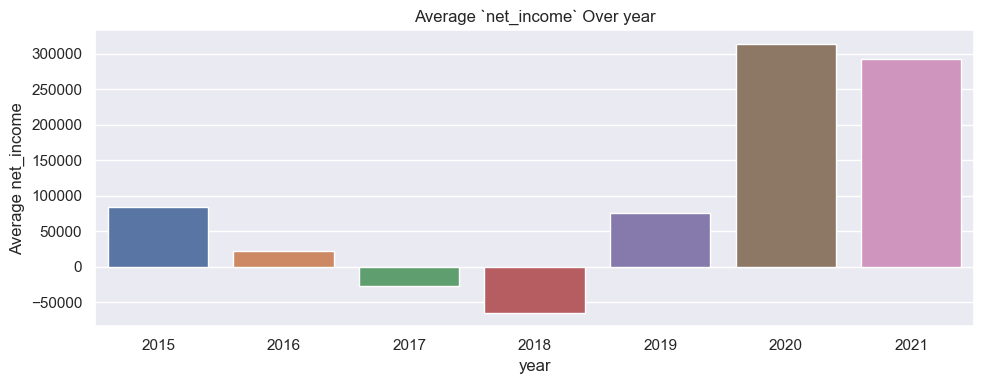
\includegraphics[width=\linewidth]{Images/netincome.png}
\caption{Total \texttt{net\_income} over time}
\label{fig:netincome EDA}
\end{figure}

\begin{figure}[htbp]
\centering
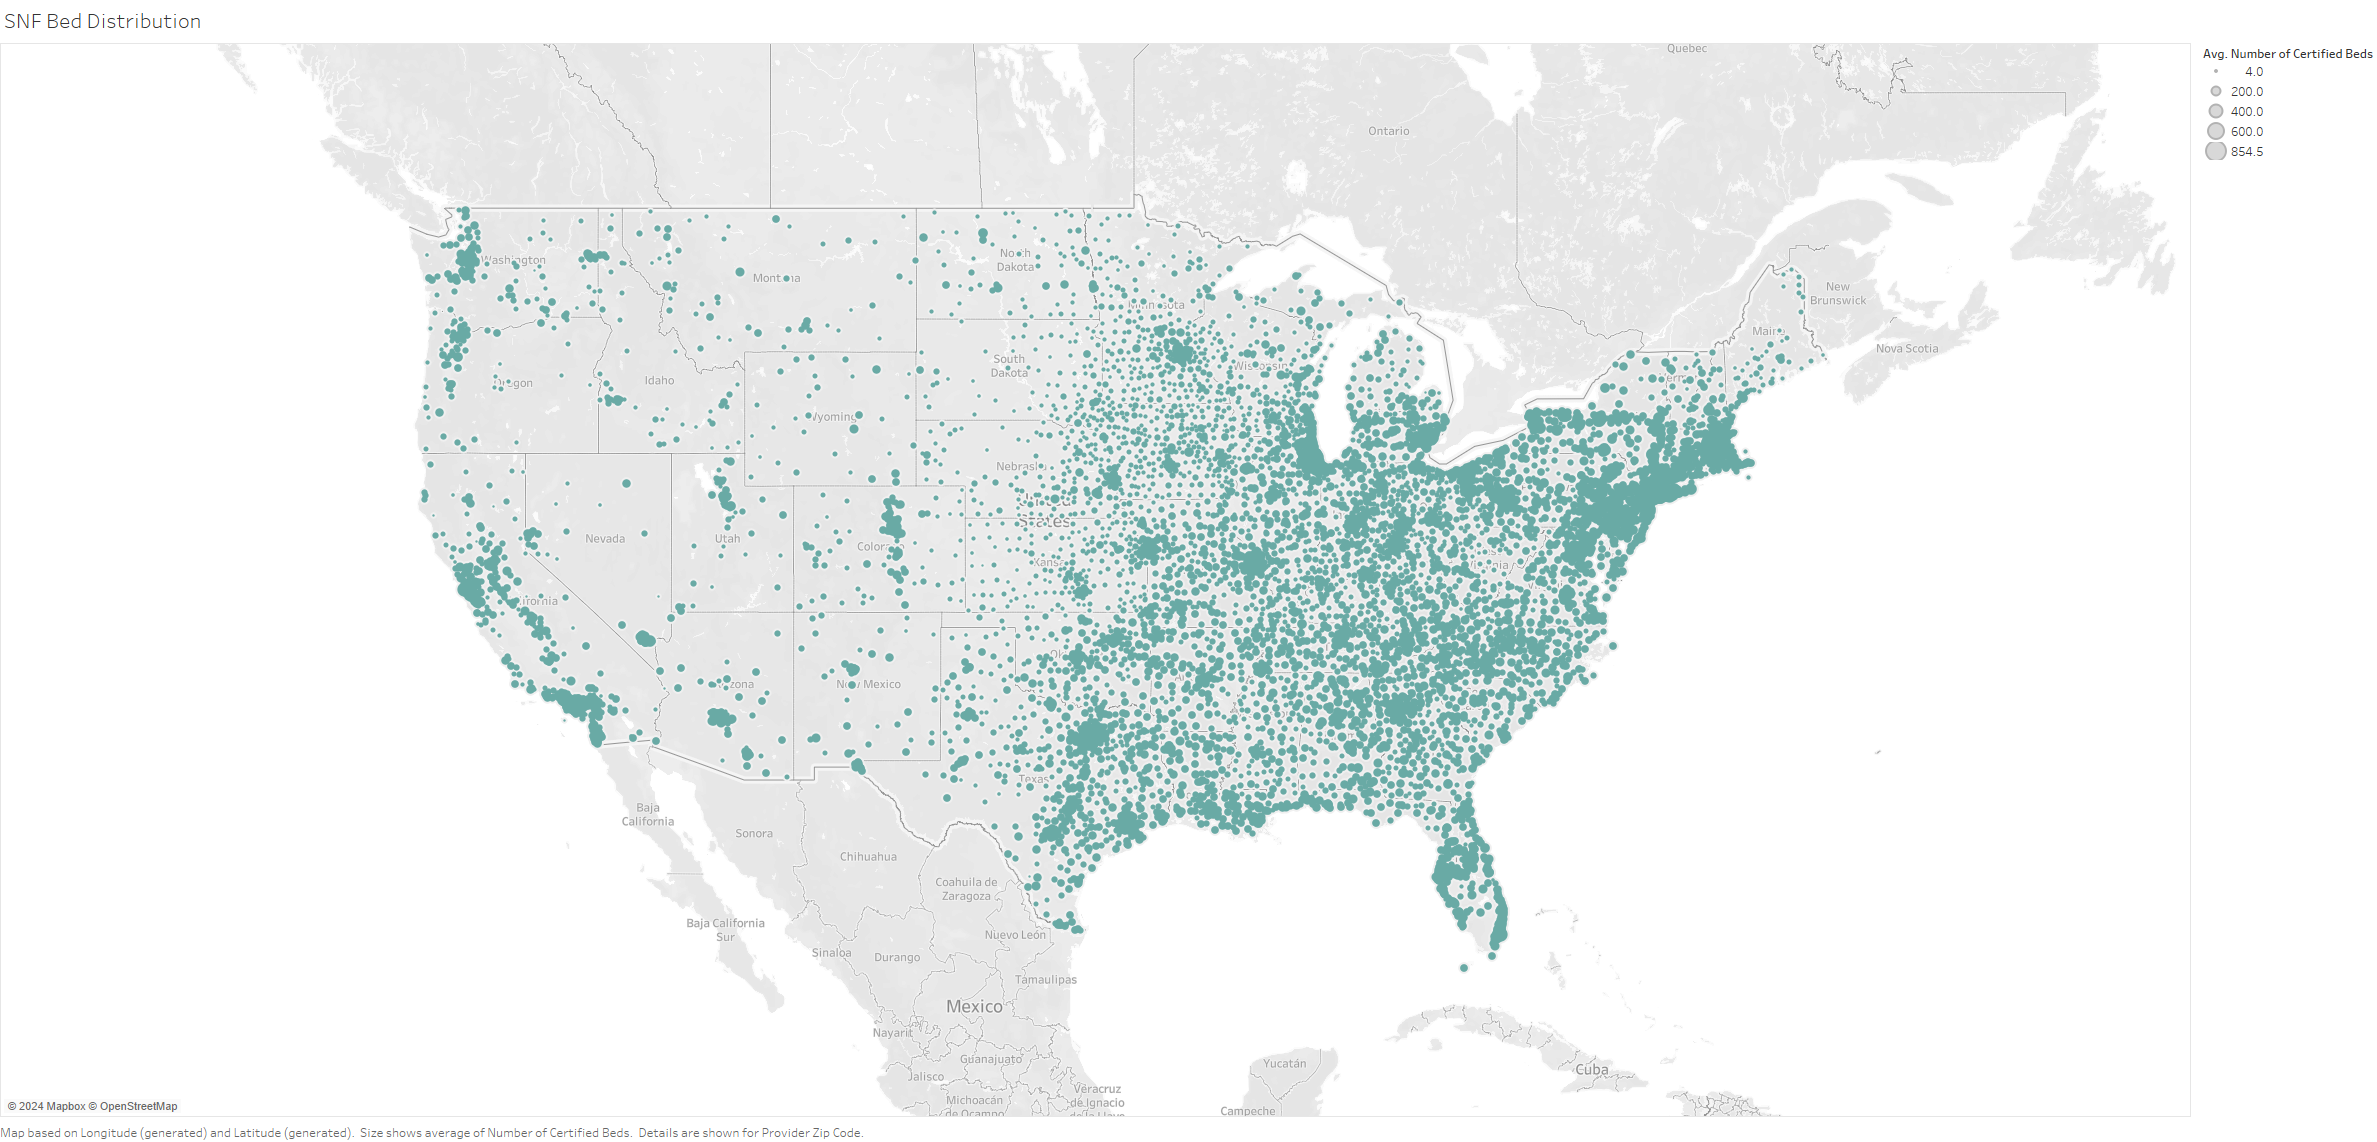
\includegraphics[width=\linewidth]{Images/SNF Bed Distribution.png}
\caption{Available SNF Bed Density by Zip Code}
\label{fig:netincome EDA}
\end{figure}

\pagebreak
\begin{figure}[!h]
\centering
\begin{minipage}{\linewidth}
    \centering % This ensures the image is centered within the minipage
    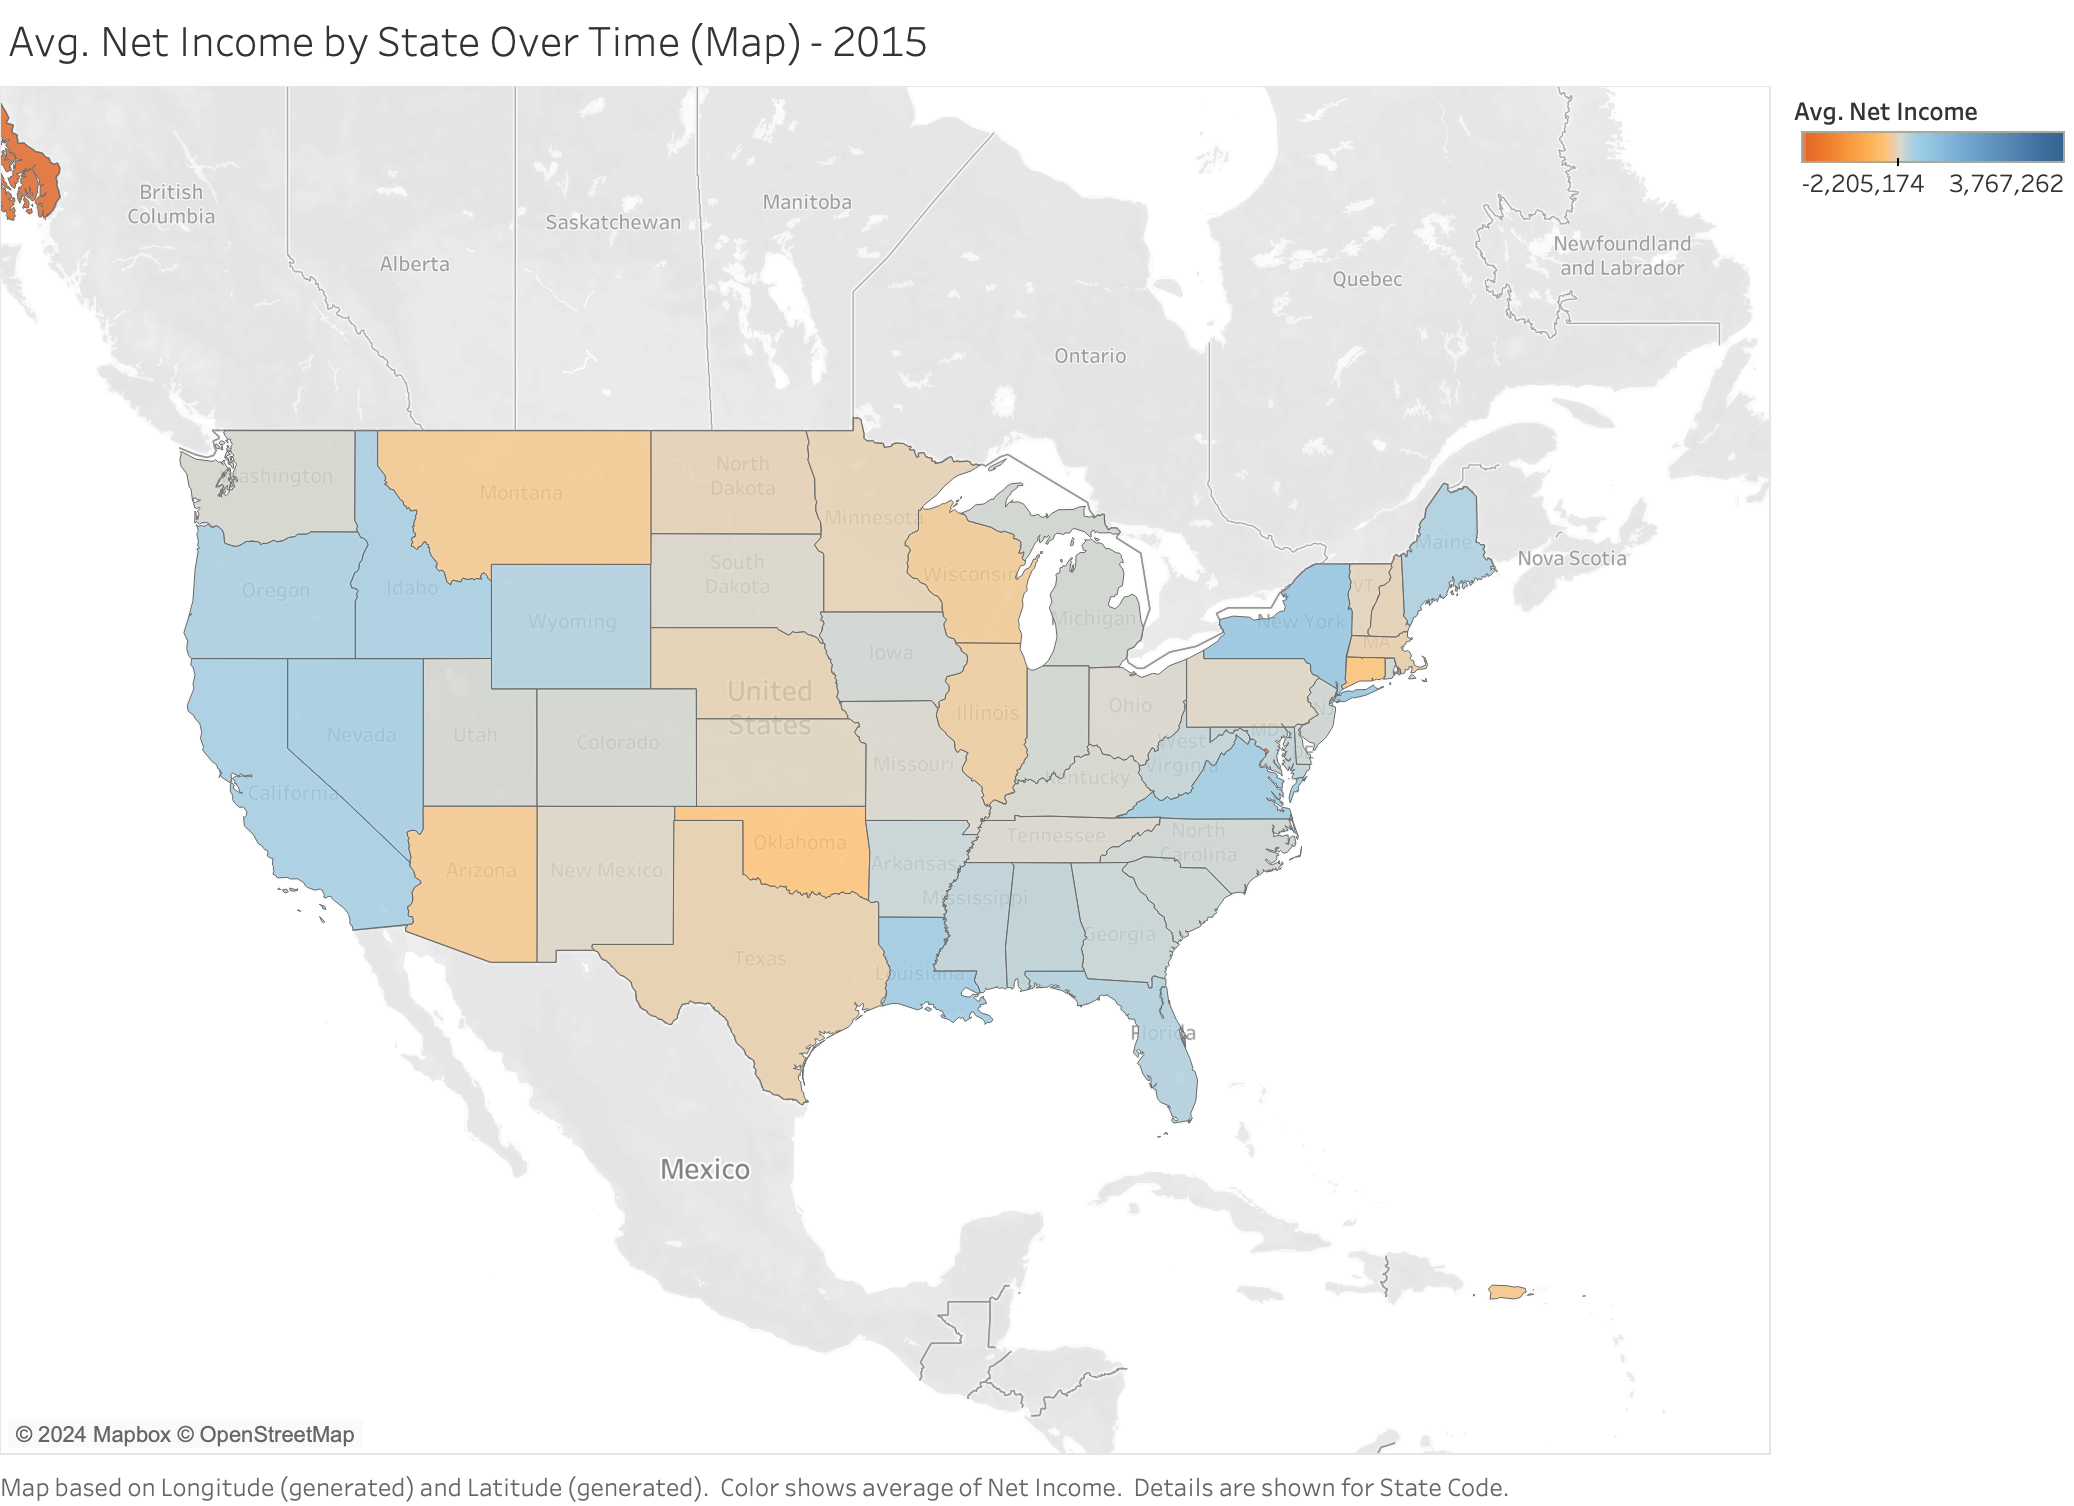
\includegraphics[width=0.75\linewidth]{Images/Avg. Net Income by State Over Time (Map).png}
    \caption{2015 - Average \texttt{net\_income} over time by State (Map)}
    \label{fig:net_income_map}
\end{minipage}\vspace{1cm} % Adds a little vertical space between the images

\begin{minipage}{\linewidth}
    \centering % This ensures the image is centered within the minipage
    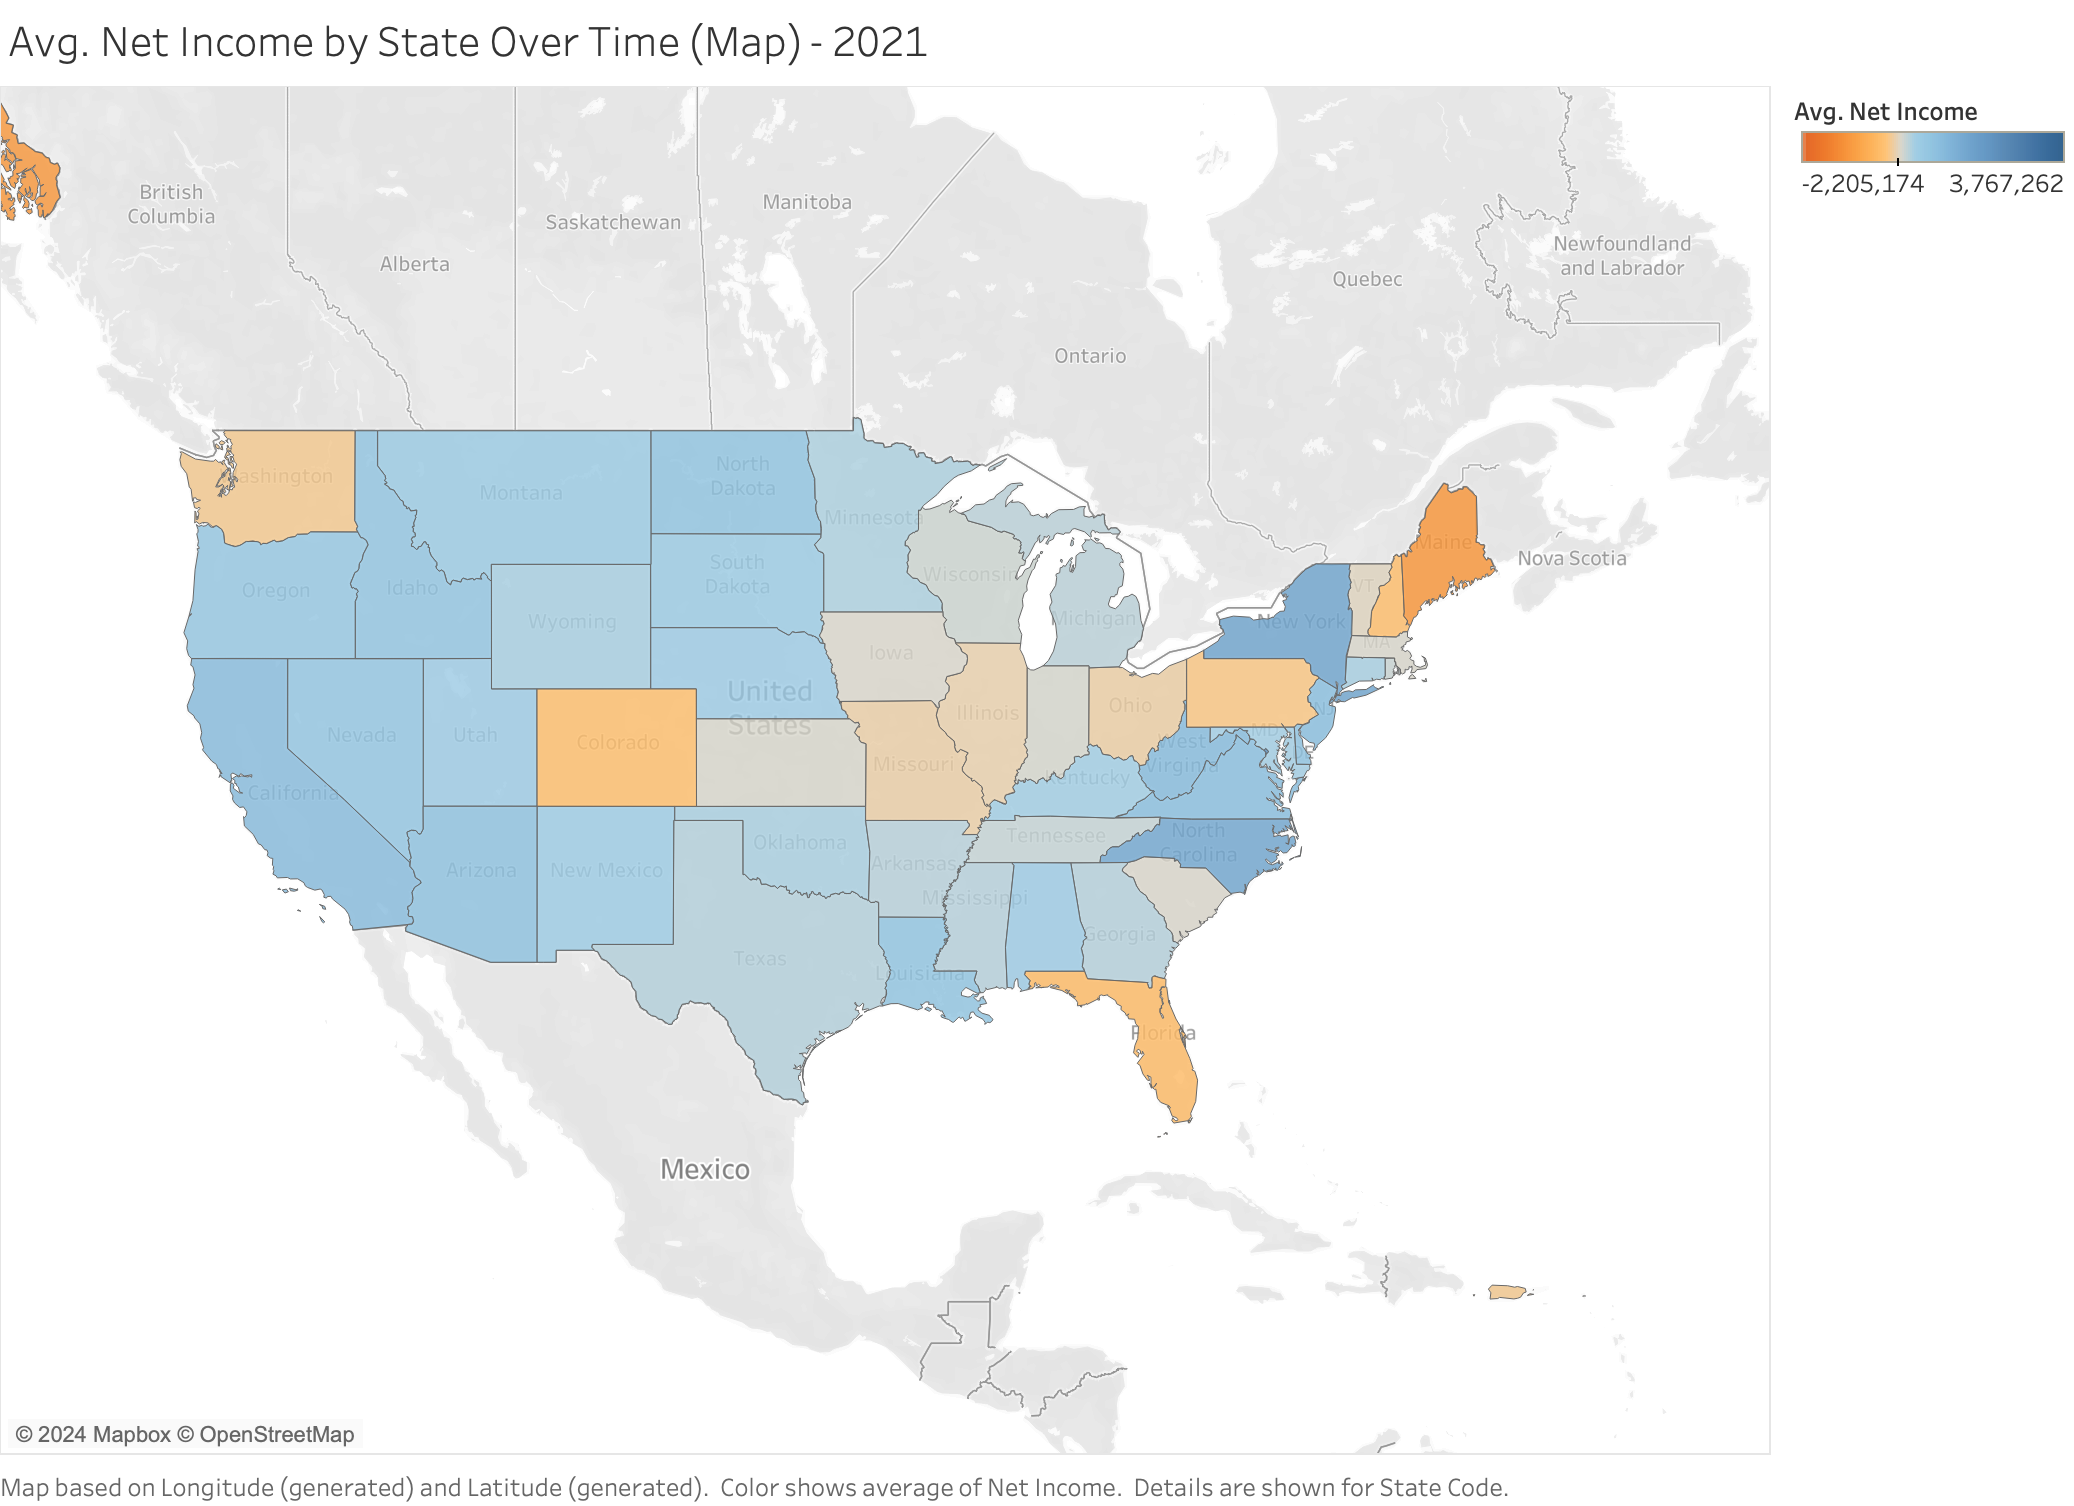
\includegraphics[width=0.75\linewidth]{Images/Avg. Net Income by State Over Time (Map)2021.png}
    \caption{2021 - Average \texttt{net\_income} over time by State (Map)}
    \label{fig:net_income_map_2021}
\end{minipage}
\end{figure}

\pagebreak

\subsection{Provider Information}
General information on currently active nursing homes, including number of certified beds, quality measure scores, staffing and other information used in the Five-Star Rating System.

CMS created the Five-Star Quality Rating System to help consumers, their families, and caregivers compare nursing homes more easily and to help identify areas about which you may want to ask questions.  The Nursing Home Care Compare web site features a quality rating system that gives each nursing home a rating of between 1 and 5 stars.  Nursing homes with 5 stars are considered to have much above average quality and nursing homes with 1 star are considered to have quality much below average.  There is one Overall 5-star rating for each nursing home, and separate ratings for health inspections, staffing and quality measure\textsuperscript{\cite{cmsfive2023}}\textsuperscript{\cite{provCMS}}. The analysis related to this dataset will attempt to determine if there exists any relationship beteen quality ratings and net income.

\subsubsection{Data Loading and Handing Missing Values}
Similar to the cost reports, this data set featured data inconsistency issues with the header names between years. The header names were made consistent with the names from 2015, and then all unmatched columns were removed. Any columns with more than 15000 null values were dropped. The data types of the numerical columns was changed to float, and since the provider number acted as the primary key, the data type of the provider number column was made consistent with the cost report data set. Once this was complete, the features net income and net profit margin were joined to the data set and any remaining records that were unable to be properly casted into the correct data type were dropped. Any records that were unable to be matched were also dropped from the dataset.

Because this data consisted of mostly scores on a one through five scale and totals, no outlier detection was applied. 

\subsubsection{Multicollinearity}
Many of the features in this data set, specifically the cycle scores and ratings, are highly correlated. This is because of their definitions; consider the following snippet from the data dictionary and correlation heatmap:

\begin{figure}[htbp]
\centering
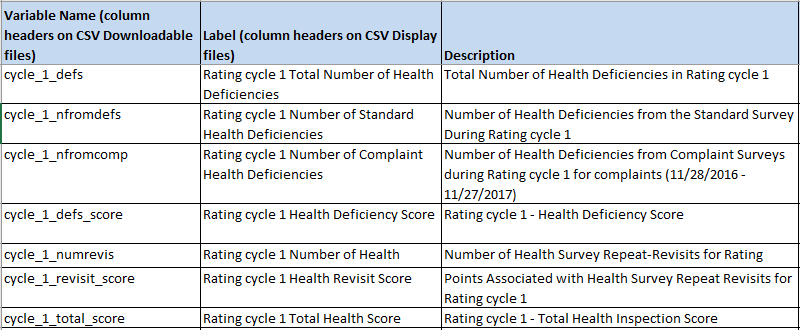
\includegraphics[width=0.8\linewidth]{Images/multicolin.png}
\caption{Data dicitonary for Cycle 1}
\label{fig:Multicolin Results}
\end{figure}

\pagebreak
\begin{figure}[htbp]
\centering
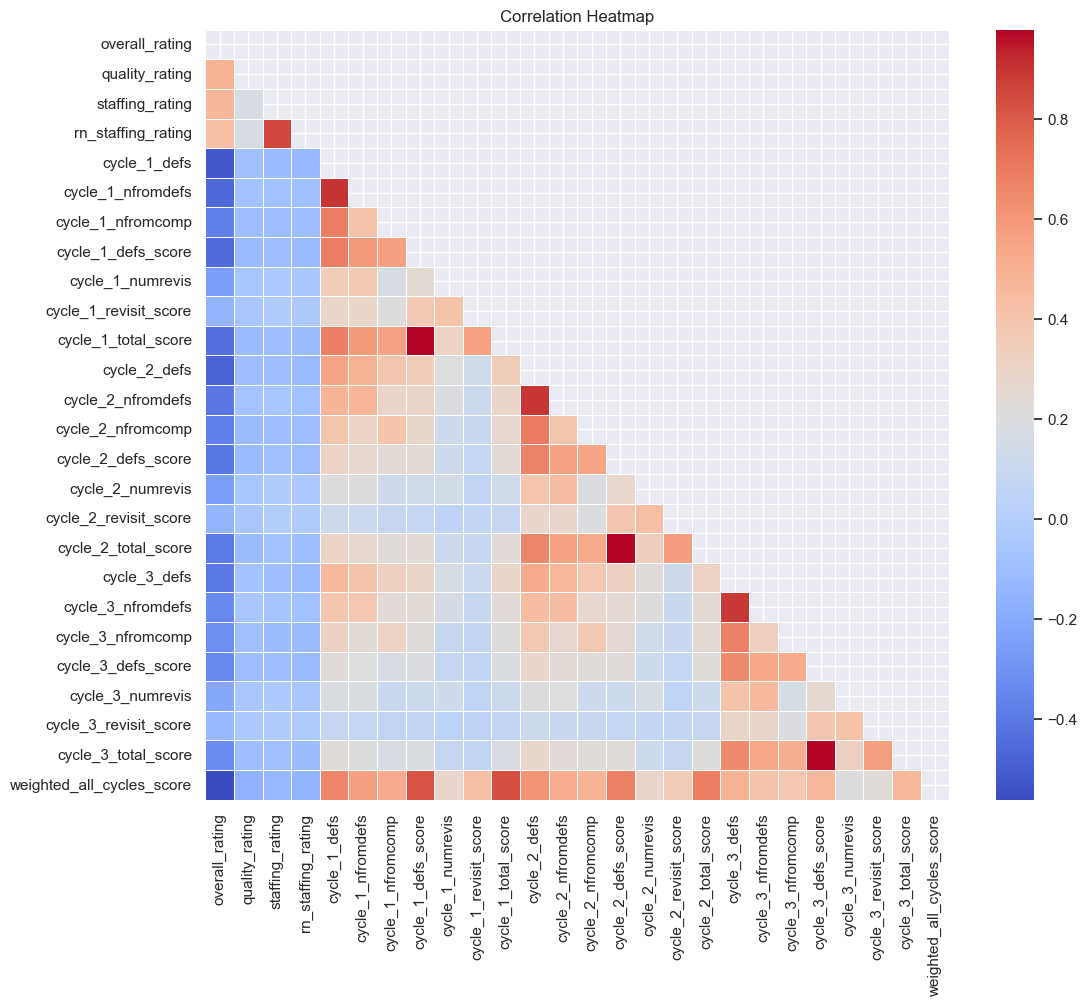
\includegraphics[width=0.8\linewidth]{Images/multicolinheat.png}
\caption{Correlation Heatmap for all columns related to ratings and cycle scores.}
\label{fig:Correl Heatmap}
\end{figure}

Including all variables in regression models will result in severe multicollinearity. Therefore, we will store highly correlated features in a drop list; we will keep the cycle totals and drop all other ratings.

\subsubsection{Exploratory Data Analysis}
After all the cleaning, we are left with a dataset in which we have the provider information and net income for each row. Using Tableau, we plotted the following features against net income: cycle score totals, weighted cycle scores, penalties, and fines. From these figures, it is clear that regression models will likely demonstrate that there does not exist any relationship between these features and net income.



\begin{figure}[htbp]
\centering
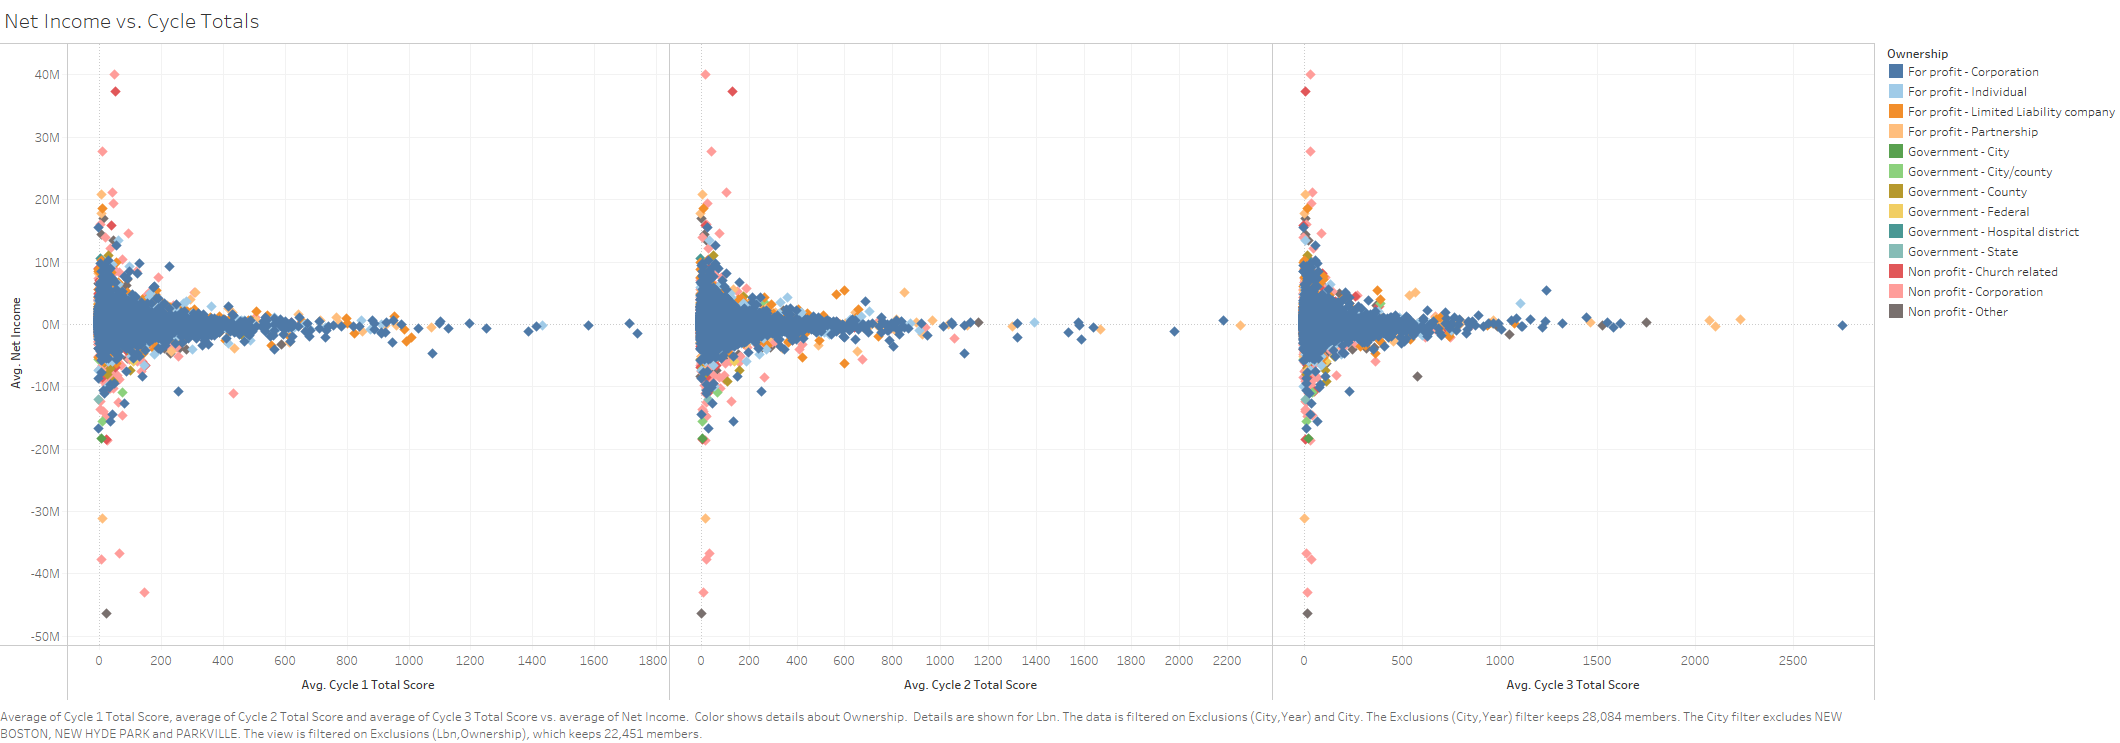
\includegraphics[width=\linewidth]{Images/Net Income vs. Cycle Totals.png}
\caption{Net income versus Cycle 1, 2, and 3 Score Totals}
\label{fig:net income vs cycle totals}
\end{figure}

\begin{figure}[htbp]
\centering
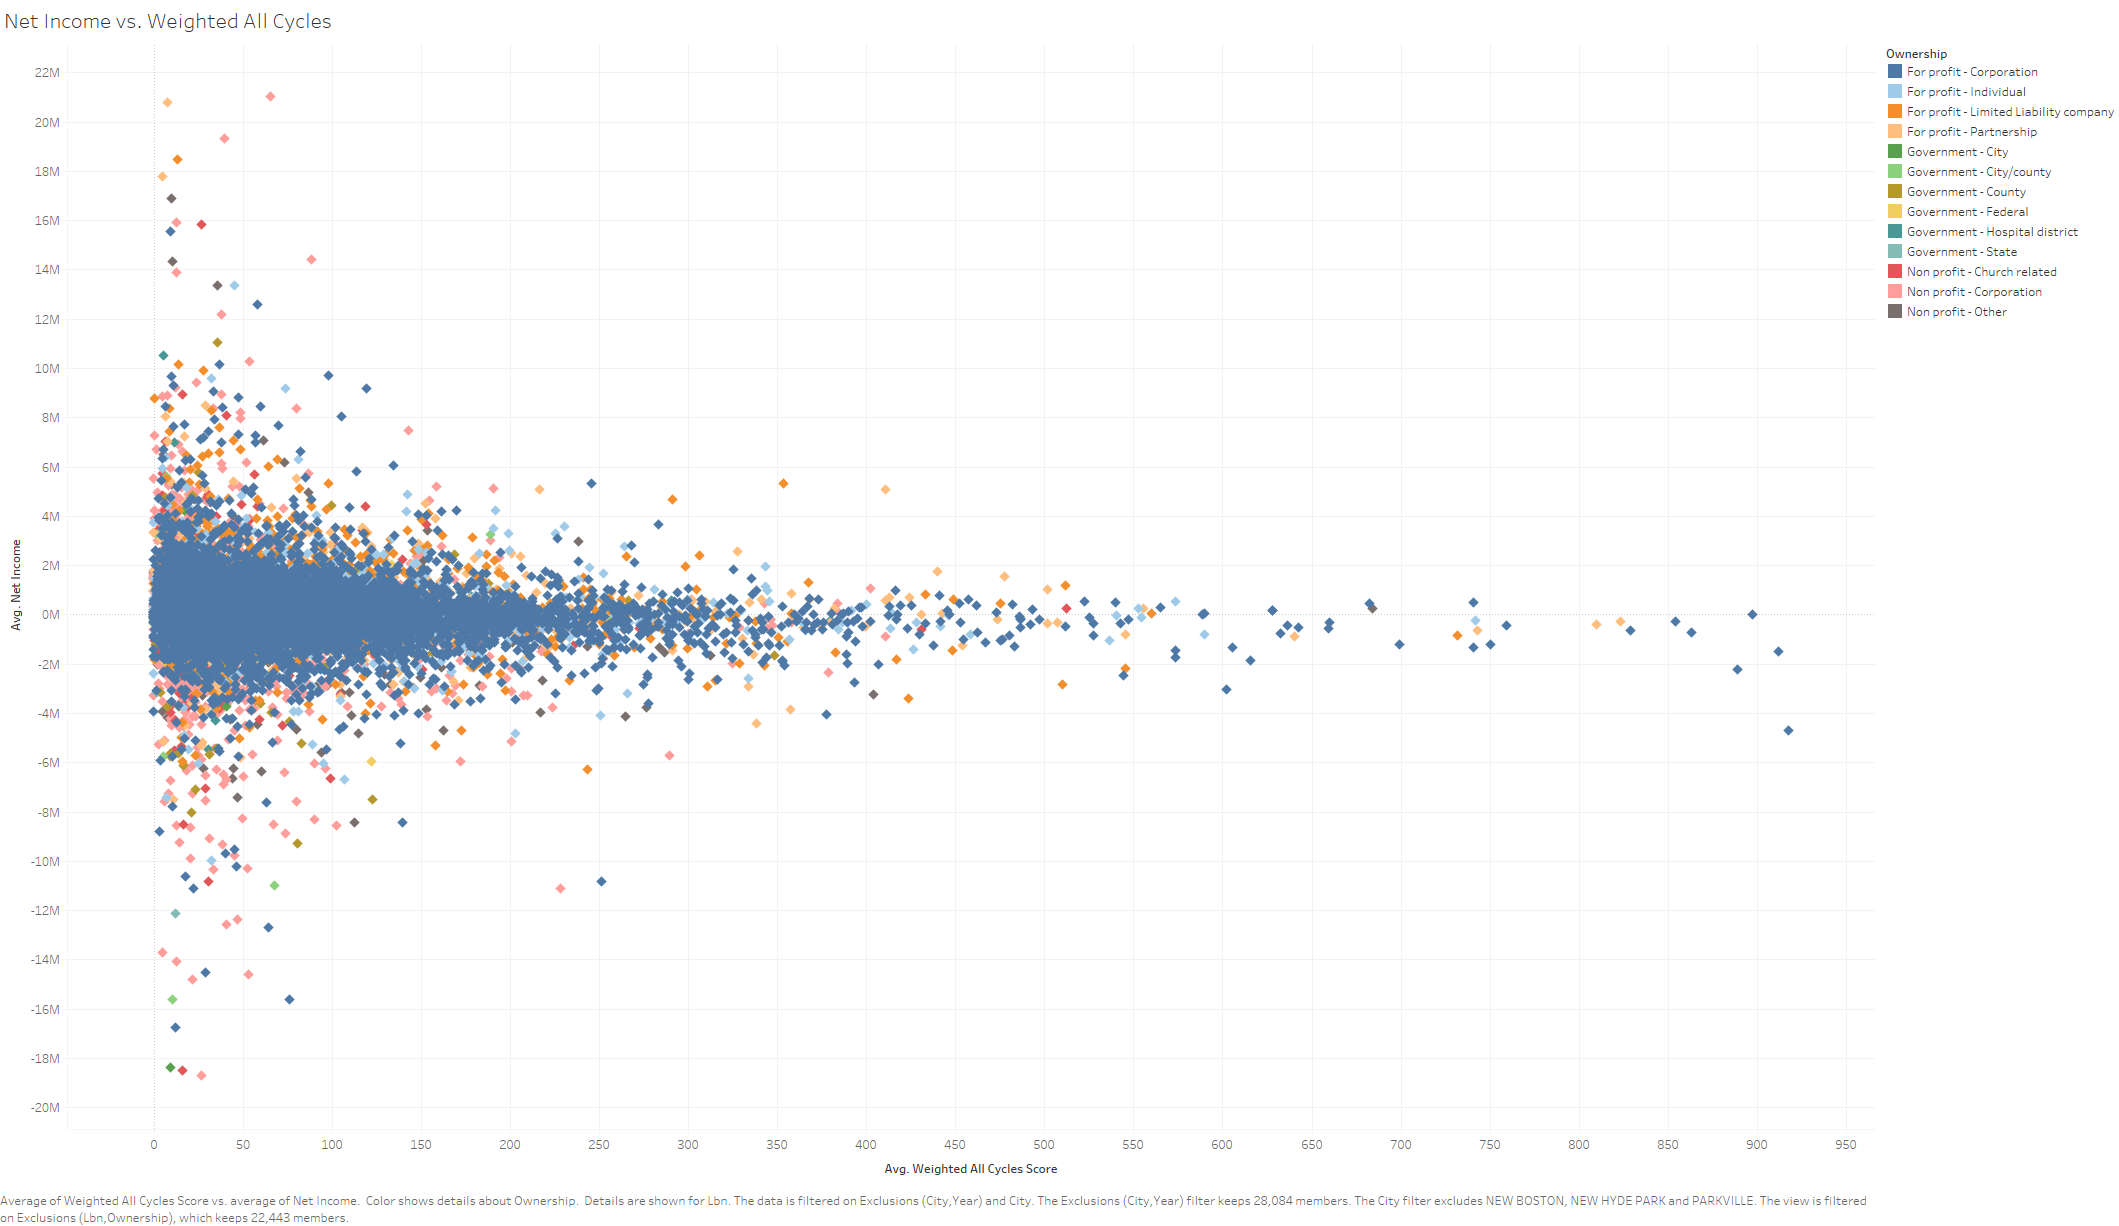
\includegraphics[width=\linewidth]{Images/Net Income vs. Weighted All Cycles.png}
\caption{Net income versus weightd all cycles score.}
\label{fig:net income vs. cycle weighted}
\end{figure}

\begin{figure}[htbp]
\centering
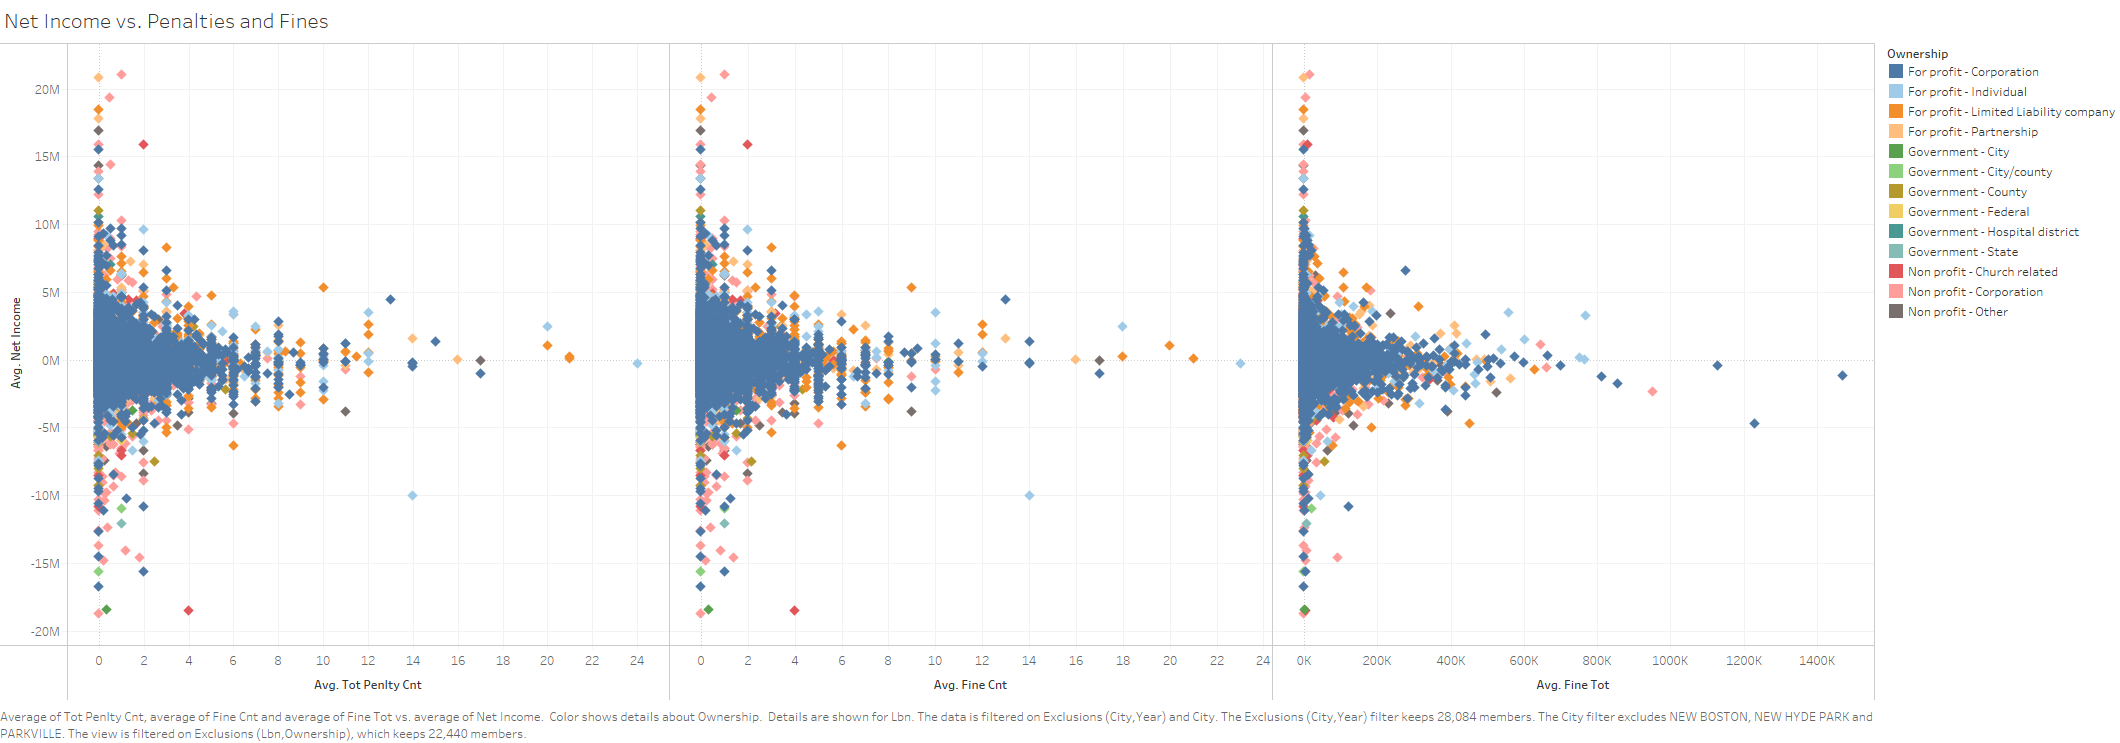
\includegraphics[width=\linewidth]{Images/Net Income vs. Penalties and Fines.png}
\caption{Net incomes versus penalties and fines.}
\label{fig:net income vs penalties and fines}
\end{figure}


\pagebreak

\subsection{COVID Vaccination Data (2021)}
Nursing homes are requried to report vaccinations of residents and staff. The Centers for Medicare \& Medicaid Services (CMS) implemented several Interim Final Rules (IFC) and a Final Rule to enforce reporting requirements for Long-Term Care (LTC) facilities. These mandates, outlined in CMS-5531-IFC and CMS-1747-F, require LTC facilities to report COVID-19 data to the National Healthcare Safety Network (NHSN) as stipulated under 42 CFR 483(g).\textsuperscript{\cite{cmsqso2313}}

The included data files for the cost reports do not contain the data for 2022. Although the COVID data for 2022 is available, only the 2021 dataset will have net income joined to the dataset. 

\subsubsection{Data Import}
The data types of all columns need to be changed, and irrelevant columns were dropped. As with the Provider data, the Federal Provider Number is the primary key that joins the financial data to our data set, hence, it needs to be of the same data type as in the cost reports (integer). Table 1 is the \texttt{info()} output upon loading, and Table 2 is the \texttt{info()} output after cleaning. 
\begin{table}[h]
\centering
\caption{CovidVax\_2021 \texttt{info()} output}
\label{tab:dataframe_structure}
\begin{tabular}{|c|l|c|}
\hline
\textbf{Column Index} & \textbf{Column Name}                               & \textbf{Data Type} \\ \hline
0                     & Federal Provider Number                            & object             \\ \hline
1                     & Provider State                                     & object             \\ \hline
2                     & Percent Vaccinated Residents                       & object             \\ \hline
3                     & Percent Vaccinated Healthcare Personnel            & object             \\ \hline
4                     & Date vaccination data last updated                 & object             \\ \hline
\end{tabular}
\end{table}


\begin{table}[h]
\centering
\caption{covid\_df \texttt{info()} output}
\label{tab:new_dataframe_structure}
\begin{tabular}{|c|l|c|}
\hline
\textbf{Column Index} & \textbf{Column Name}                               & \textbf{Data Type} \\ \hline
0                     & provnum                                            & int32              \\ \hline
1                     & Percent Vaccinated Residents                       & float64            \\ \hline
2                     & Percent Vaccinated Healthcare Personnel            & float64            \\ \hline
3                     & net\_income                                        & float64            \\ \hline
\end{tabular}
\end{table}


\subsubsection{Exploratory Data Analysis}
The plots below aim to help examine the relationship between net income and vaccination rates of nursing homes. From the analyses of these plots, it is evident that while there is a positive correlation between the vaccination rates of residents and personnel, the net income and vaccination rates do not show a straightforward relationship.
\begin{figure}[htbp]
\centering
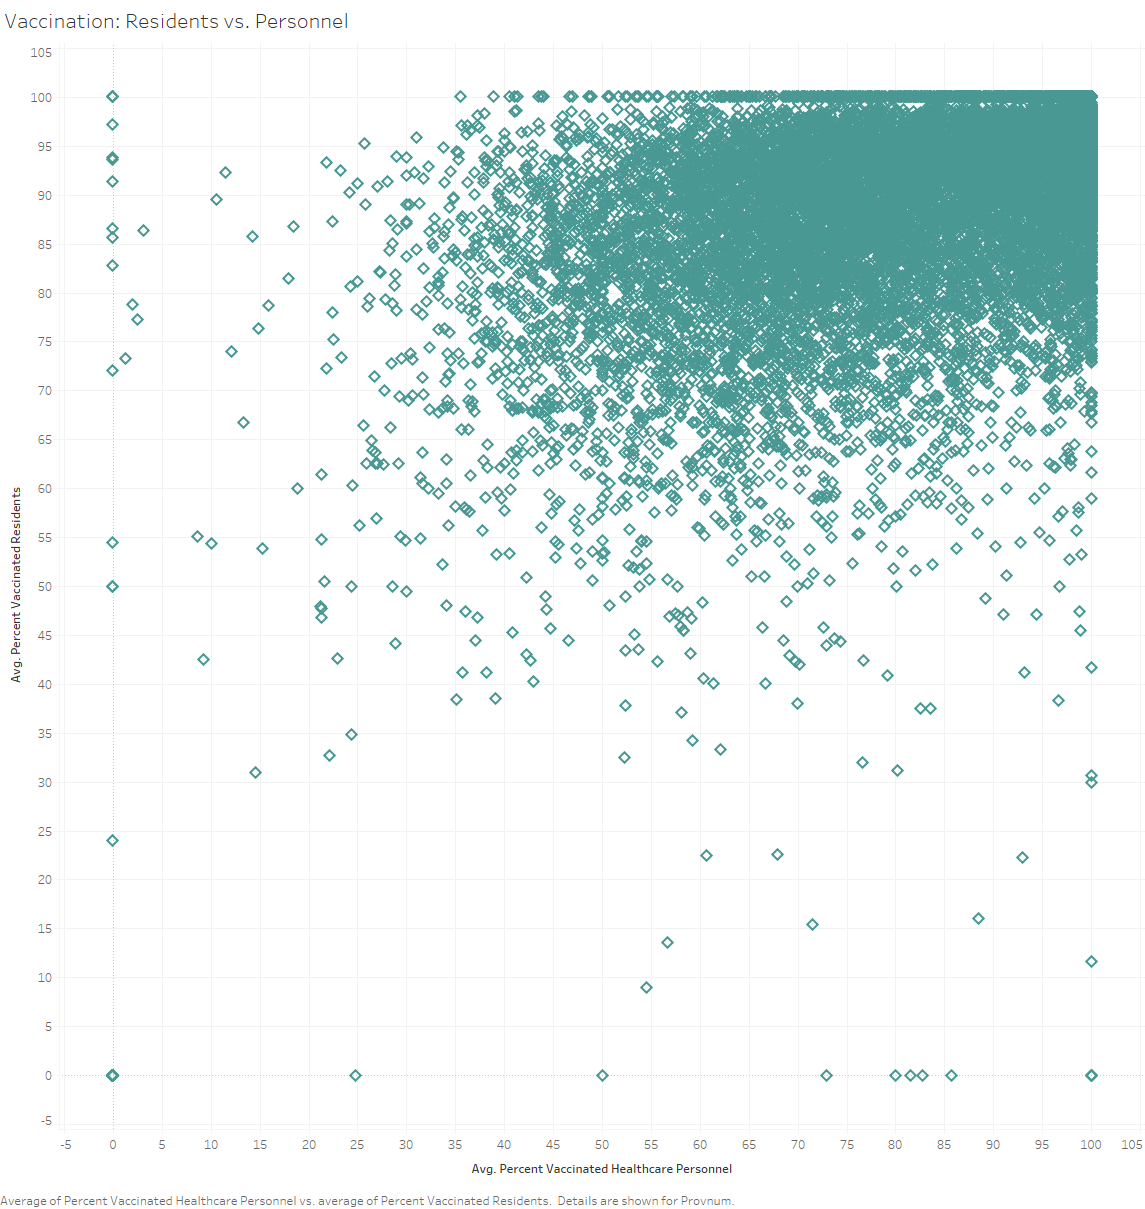
\includegraphics[width=0.6\linewidth]{Images/Vaccination Residents vs. Personnel.png}
\caption{Vaccination of residents versus personnel}
\label{fig:vaccination scatterplot}
\end{figure}

\begin{figure}[htbp]
\centering
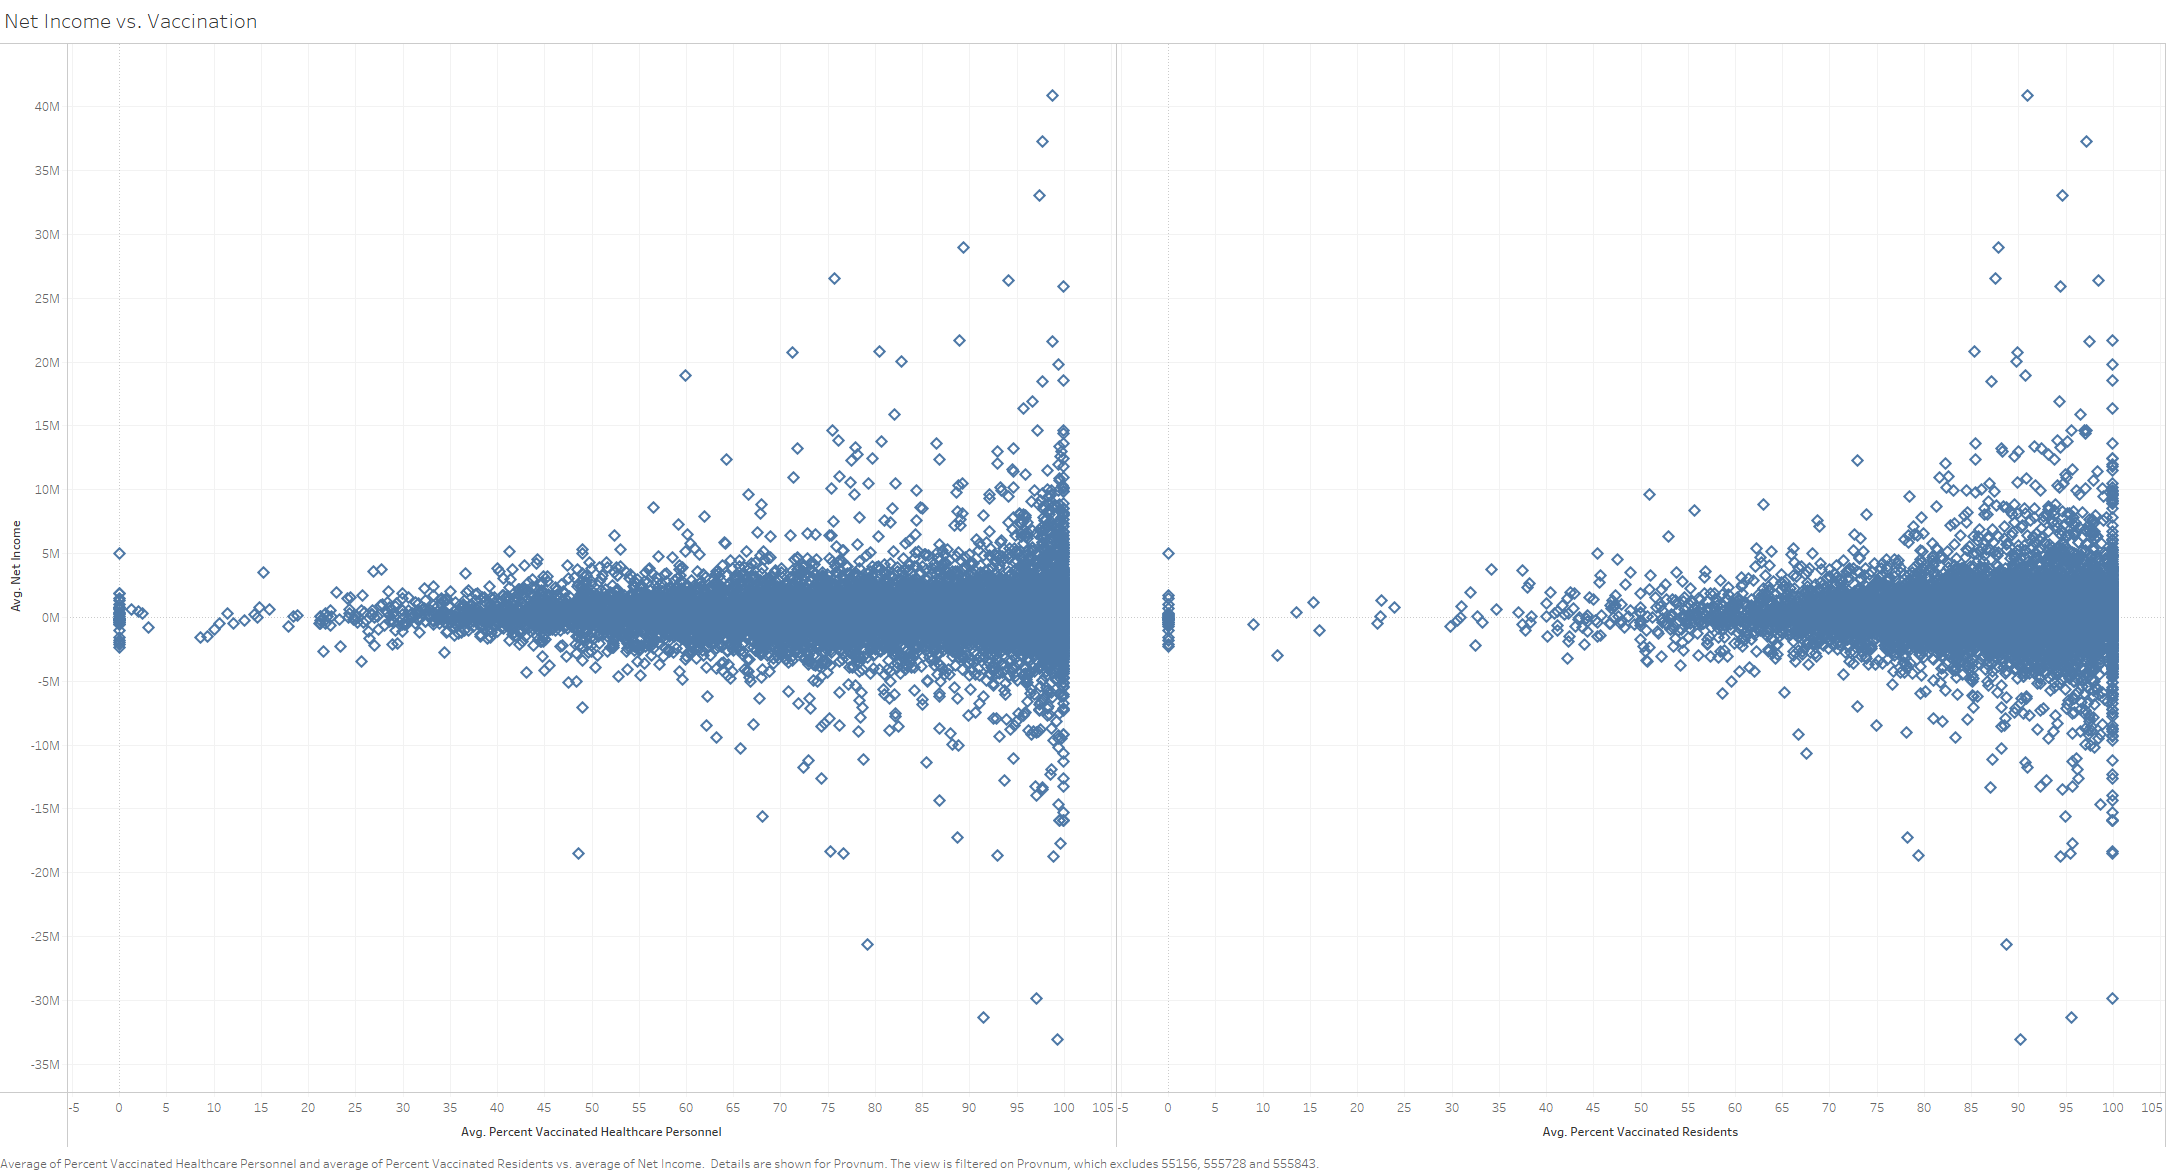
\includegraphics[width=\linewidth]{Images/Net Income vs. Vaccination.png}
\caption{Net income versus vaccination of both residents and personnel}
\label{fig:net income vs vacc}
\end{figure}

\pagebreak

%-------------------BEGIN: Analysis and Findings------------------------------------
\section{Analysis and Findings}

Models were were developed and ran against the cost report data, the provider information data, and the COVID data. The sections below detail the model building process and the analysis from each model.

\subsection{Model Fit and Comparison for Cost Report Dataset}
The analysis incorporated two distinct normalization techniques: \texttt{StandardScaler()} and \texttt{RobustScaler()}. These scalers were selected to evaluate the robustness and performance of the models under different scaling conditions. The regression algorithms employed in the study included Linear Regression, Lasso Regression, Ridge Regression, Elastic Net Regression, and K-Nearest Neighbors Regression. Each model was systematically applied to the dataset after the application of each scaler to determine the impact on the predictive accuracy. The implementation of these models is detailed below:

\begin{lstlisting}[language=Python, caption=Regression model pipeline code]
def evaluate_regression_models(df, target_column, scaler, test_size=0.1, random_state=123):
    """
    Evaluate various regression models on a given DataFrame with specified scaler.

    Parameters:
    - df : DataFrame containing the data.
    - target_column : string, the name of the column to predict.
    - scaler : Scaler object from sklearn.preprocessing.
    - test_size : float, the proportion of the dataset to include in the test split.
    - random_state : int, random_state is the seed used by the random number generator.
    """
    
    X = df.drop([target_column], axis=1)
    y = df[target_column]

    # Define numerical features for scaling
    numericalFeatures = X.columns[X.dtypes != 'object']

    # Preprocessor using ColumnTransformer to apply scaling only to numerical features
    preprocessor = ColumnTransformer(
        transformers=[
            ('num', scaler, numericalFeatures)
        ])

    models = {
        'Linear Regression': LinearRegression(),
        'Ridge': Ridge(alpha=20000),
        'Lasso': Lasso(alpha=20000),
        'ElasticNet': ElasticNet(alpha=1.0, l1_ratio=0.5),
        'KNN': KNeighborsRegressor(n_neighbors=2)
    }

    results = pd.DataFrame(index=models.keys(), columns=['Mean Squared Error', 'R-squared', 'Adjusted R-squared'])

    # Iterate over models, create a full pipeline, and evaluate
    for name, model in models.items():
        pipeline = Pipeline(steps=[('preprocessor', preprocessor),
                                   ('regressor', model)])
        # Split data into train and test sets
        X_train, X_test, y_train, y_test = train_test_split(X, y, test_size=test_size, random_state=random_state)
        # Fit the model
        pipeline.fit(X_train, y_train)
        # Predict
        y_pred = pipeline.predict(X_test)
        # Evaluate
        mse = mean_squared_error(y_test, y_pred)
        r2 = r2_score(y_test, y_pred)
        n = len(X_train)
        p = len(X.columns)
        adj_R2 = 1- ((1-r2) * (n-1)/(n-p-1))
        results.loc[name] = [mse, r2, adj_R2]

    print(results)

    # Plotting results
    fig, ax = plt.subplots(1, 2, figsize=(14, 6))
    results.plot(kind='bar', y='Adjusted R-squared', ax=ax[0], color='skyblue', title=f'Adjusted R-Squared by Model (Scaler: {scaler})')
    results.plot(kind='bar', y='R-squared', ax=ax[1], color='orange', title=f'R-squared by Model (Scaler: {scaler})')
    plt.tight_layout()
    plt.show()
\end{lstlisting}

The code above was built in a way such that it would be quick to apply to the different datasets related to this project. 

\pagebreak

\subsubsection{Comparing Model Performance}

The performance of various regression models on the dataset is summarized in the figures and tables below. The metrics used for evaluation are the coefficient of determination (R-squared) and adjusted R-squared. The formula used for calculating adjusted r-squared is below. Mean squared error results are contained in the codebase repository, for refenece. 



    \[
R_{\text{adjusted}}^2 = 1 - (1 - R^2) \frac{n - 1}{n - p - 1}\]

where:
\begin{itemize}
    \item $R^2$ is the coefficient of determination.
    \item $n$ is the sample size in the training data.
    \item $p$ is the number of features in the model.
\end{itemize}

\begin{lstlisting}[language=Python, caption=R-squared computation within evaluation function]
        r2 = r2_score(y_test, y_pred)
        n = len(X_train)
        p = len(X.columns)
        adj_R2 = 1- ((1-r2) * (n-1)/(n-p-1))
\end{lstlisting}


\begin{figure}[htbp]
\centering
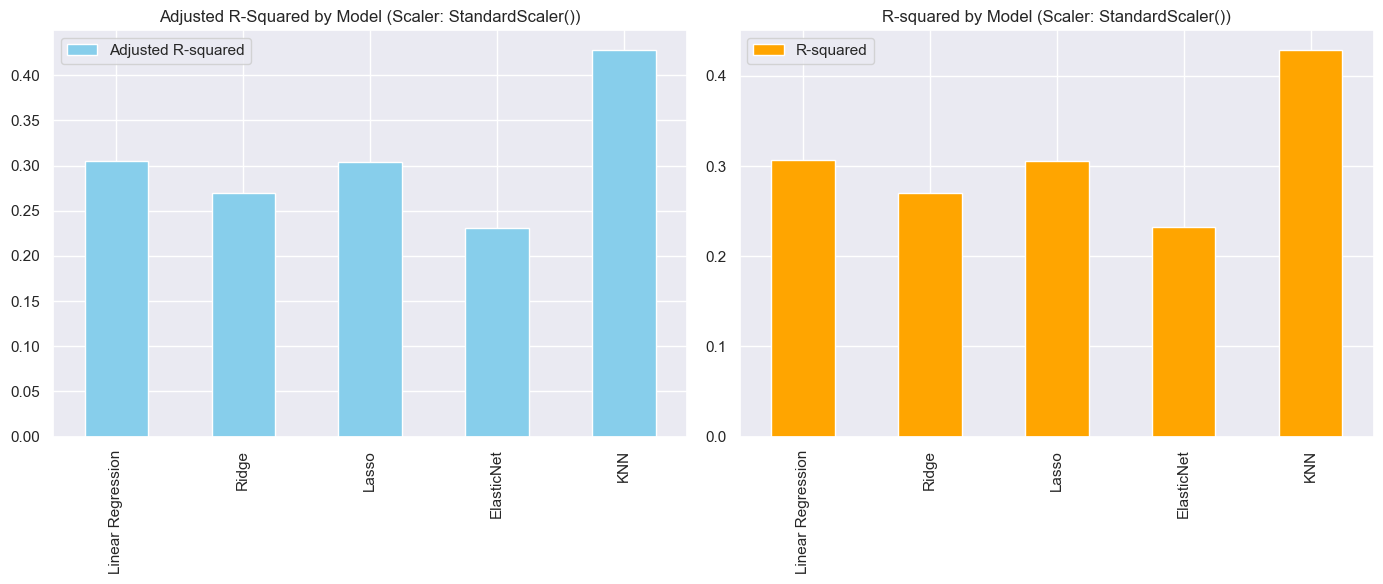
\includegraphics[width=\linewidth]{./Images/evalRegModelStandardScaler.png}
\caption{Results for \texttt{StandardScaler()}}
\label{fig:Standard Scaler Results}
\end{figure}

\begin{table}[ht]
\centering
\begin{tabular}{@{}lrr@{}}
\toprule
Model & \multicolumn{1}{c}{R-squared} & \multicolumn{1}{c}{Adjusted R-squared} \\ 
\midrule
Linear Regression & 0.30621 & 0.30541 \\
Ridge & 0.27029 & 0.26945 \\
Lasso & 0.30511 & 0.30431 \\
ElasticNet & 0.23217 & 0.23128 \\
KNN & 0.42898 & 0.42833 \\
\bottomrule
\end{tabular}
\label{tab:model_performance_updated_standard_scaler}
\end{table}

\FloatBarrier % Prevent floats from moving past this point
\pagebreak

\begin{figure}[htbp]
\centering
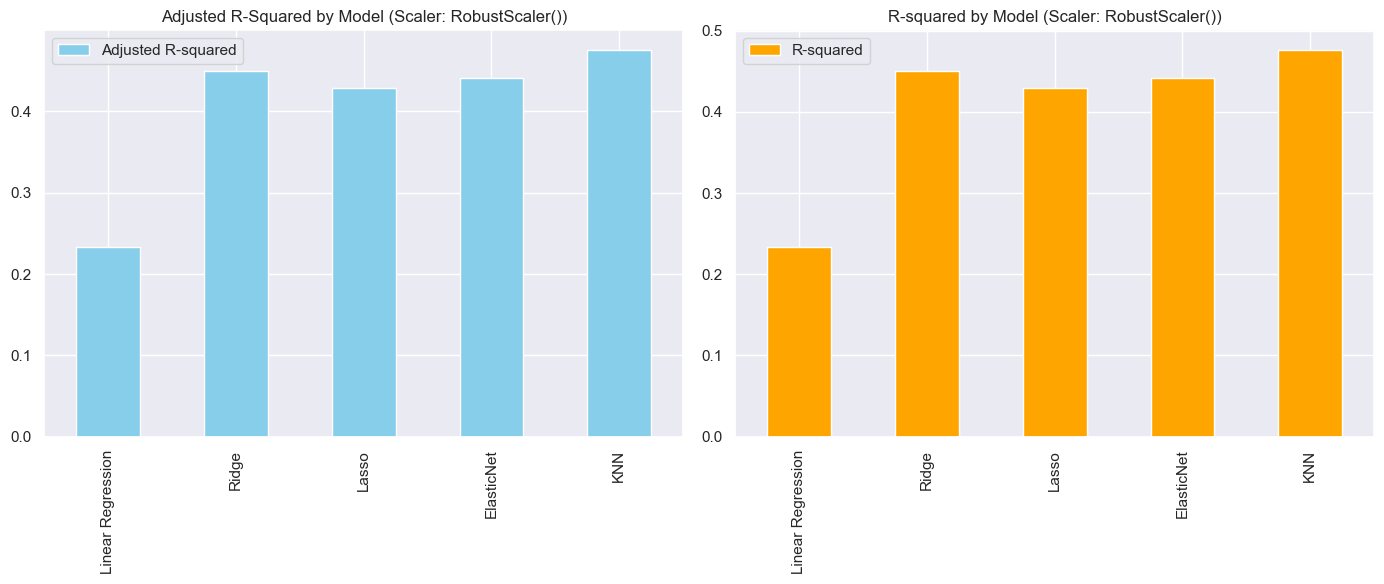
\includegraphics[width=\linewidth]{Images/evalRegModelRobustScaler.png}
\caption{Results for \texttt{RobustScaler()}}
\label{fig:Robust Scaler Results}
\end{figure}


\begin{table}[ht]
\centering
\begin{tabular}{@{}lrr@{}}
\toprule
Model             & \multicolumn{1}{c}{R-squared} & \multicolumn{1}{c}{Adjusted R-squared} \\ 
\midrule
Linear Regression  & 0.30619 & 0.30539 \\
Ridge              & 0.29729 & 0.29649 \\
Lasso              & 0.29982 & 0.29901 \\
ElasticNet         & 0.29437 & 0.29356 \\
KNN                & 0.45196 & 0.45133 \\
\bottomrule
\end{tabular}
\label{tab:model_performance_updated}
\end{table}

\FloatBarrier % Another barrier to keep subsequent sections or floats in place

All models perform closely, with linear Regression and KNN performing the best. Additionally, we notice that all models performed similar when utilizing \texttt{RobustScaler()} as opposed to \texttt{StandardScaler()}. Furthermore, given that R-squared and adjusted R-squared are close, we can determine that the model is balanced in terms of complexity and capability. 

Although KNN was the best performing model, because of it's nature it is difficult to determine which features are most important. Because linear regression was the best performing parametric model, this is the model we will go with to analyze feature importance. 
\pagebreak

\subsubsection{Regression Coefficients}

In quantitative analysis via linear regression with standardized features, the magnitude and sign of the model's coefficients are indicative of the predictors' association with the target variable—net income of nursing homes. Higher absolute values denote stronger influence, with positive coefficients suggesting an increasing relationship, and negative ones indicating a decreasing effect. Given this, we can determine the most important features by extracting the coefficient values from the model:


\begin{table}[ht]
\centering
\caption{Top 16 Important Features and Their Coefficients}
\begin{tabular}{@{}cll@{}}
\toprule
Rank & Feature & Coefficient \\
\midrule
1 & state\_code\_AK & -1,191,000.373 \\
2 & total\_assets & 756,958.354 \\
3 & state\_code\_HI & 744,647.905 \\
4 & inpatient\_pps\_amount & 629,854.187 \\
5 & overhead\_non\_salary\_costs & -567,719.686 \\
6 & state\_code\_MA & -547,103.895 \\
7 & state\_code\_CT & -474,253.284 \\
8 & state\_code\_WV & 465,717.309 \\
9 & total\_liab\_and\_fund\_balances & -460,794.051 \\
10 & state\_code\_PR & 409,564.906 \\
11 & less\_total\_operating\_expense & -398,164.518 \\
12 & total\_salaries\_adjusted & 378,965.722 \\
13 & state\_code\_NY & 356,660.838 \\
14 & state\_code\_DE & 356,255.447 \\
15 & state\_code\_OR & 354,375.534 \\
16 & net\_profit\_margin & 347,998.182 \\
\bottomrule
\end{tabular}
\label{tab:important_features}
\end{table}

\begin{table}[ht]
\centering
\caption{Important Non-State Features and Their Impact on Net Income}
\begin{tabular}{@{}cll@{}}
\toprule
Rank & Feature & Coefficient \\
\midrule
2 & total\_assets & 756,958.354 \\
4 & inpatient\_pps\_amount & 629,854.187 \\
5 & overhead\_non\_salary\_costs & -567,719.686 \\
9 & total\_liab\_and\_fund\_balances & -460,794.051 \\
11 & less\_total\_operating\_expense & -398,164.518 \\
12 & total\_salaries\_adjusted & 378,965.722 \\
16 & net\_profit\_margin & 347,998.182 \\
23 & total\_days\_title\_xviii & -255,751.032 \\
24 & total\_general\_inpatient\_revenue & 237,721.308 \\
32 & cost\_per\_bed & -180,931.862 \\
33 & total\_days\_total & 179,750.310 \\
35 & total\_liabilities & -176,858.834 \\
37 & salary\_costs\_per\_bed & 147,008.712 \\
41 & total\_costs & -131,732.351 \\
42 & less\_discounts\_on\_patients & 114,242.849 \\
\bottomrule
\end{tabular}
\label{tab:non_state_important_features}
\end{table}
\pagebreak


\subsubsection{Cluster Analysis}
This section of the report presents a comprehensive analysis aimed at understanding the market of skilled nursing facilities across various states. Utilizing the previously ocmpleted regression analysis, we use clustering techniques to create distinct segments of skilled nursing facilities by state. We use Analysis of Variance (ANOVA) to ascertain the statistical significance of these variables. The data below uses the most recent cost report data avaiable from 2021. 
\begin{figure}[htbp]
\centering
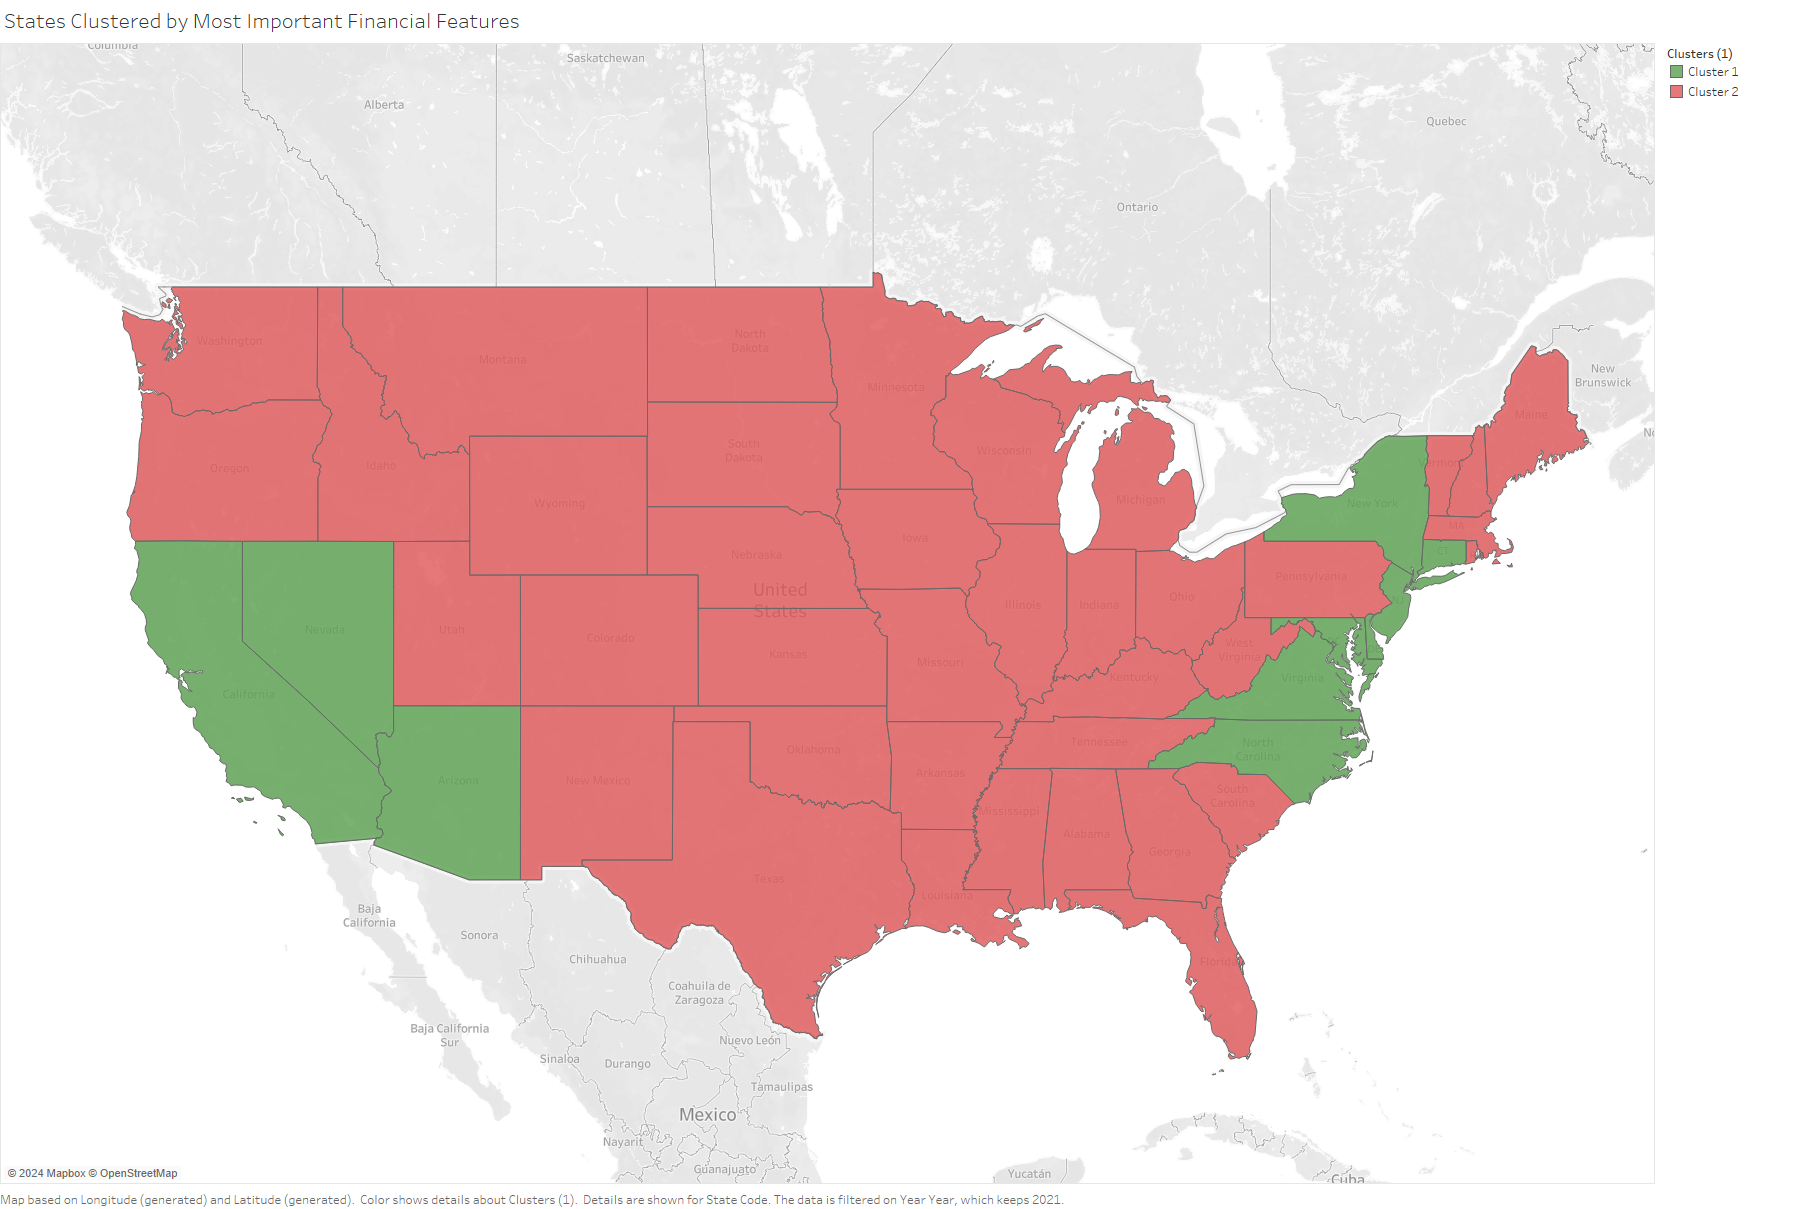
\includegraphics[width=\linewidth]{Images/States Clustered by Most Important Financial Features.png}
\caption{States clustered by 7 most important financial features}
\label{fig:Clustering}
\end{figure}

\noindent Twelve states were placed into cluster 1 and all other states were placed into cluster 2. Below are exactly the outputs from Tableau's clustering generation. 

\subsection*{Cluster 1 - State Codes}
\begin{tabular}{@{}c@{}}
\toprule
\textbf{State Code} \\
\midrule
AZ \\
CA \\
CT \\
DC \\
DE \\
HI \\
MD \\
NC \\
NJ \\
NV \\
NY \\
VA \\
\bottomrule
\end{tabular}



\subsection*{Inputs for Clustering}
\begin{itemize}
    \item \textbf{Variables:}
    \begin{itemize}
        \item Avg. Inpatient Pps Amount
        \item Avg. Less Total Operating Expense
        \item Avg. Net Income
        \item Avg. Net Profit Margin
        \item Avg. Overhead Non Salary Costs
        \item Avg. Total Assets
        \item Avg. Total Salaries Adjusted
    \end{itemize}
    \item \textbf{Level of Detail:} State Code
    \item \textbf{Scaling:} Normalized
\end{itemize}


\subsection*{Analysis of Variance (ANOVA)}
\begin{tabular}{@{}lllllll@{}}
\toprule
\textbf{Variable} & \textbf{F-statistic} & \textbf{p-value} & \textbf{Model SS} & \textbf{DF} & \textbf{Error SS} & \textbf{DF} \\
\midrule
Avg. Inpatient Pps Amount & 24.94 & 7.909e-06 & 0.8387 & 1 & 1.648 & 49 \\
Avg. Overhead Non Salary Costs & 21.64 & 2.527e-05 & 0.8122 & 1 & 1.839 & 49 \\
Avg. Net Income & 21.39 & 2.767e-05 & 0.6827 & 1 & 1.564 & 49 \\
Avg. Total Salaries Adjusted & 20.53 & 3.783e-05 & 0.7981 & 1 & 1.905 & 49 \\
Avg. Less Total Operating Expense & 20.52 & 3.8e-05 & 0.7824 & 1 & 1.869 & 49 \\
Avg. Net Profit Margin & 6.836 & 0.01184 & 0.328 & 1 & 2.351 & 49 \\
Avg. Total Assets & 3.428 & 0.07012 & 0.08364 & 1 & 1.195 & 49 \\
\bottomrule
\end{tabular}

\section*{Clustering Summary}
\noindent\textbf{Number of Clusters:} 2 \\
\textbf{Number of Points:} 51 \\
\textbf{Between-group Sum of Squares:} 4.3257 \\
\textbf{Within-group Sum of Squares:} 8.0459 \\
\textbf{Total Sum of Squares:} 12.372

\subsection*{Cluster Centers}

\begin{tabular}{@{}ll@{}}
\toprule
\textbf{Cluster} & \textbf{1} \\
\midrule
\textbf{Number of Items} & 12 \\
\textbf{Avg. Inpatient Pps Amount} & \$3.2005M \\
\textbf{Avg. Less Total Operating Expense} & \$15.684M \\
\textbf{Avg. Net Income} & \$1.0658M \\
\textbf{Avg. Net Profit Margin} & 4.4611\% \\
\textbf{Avg. Overhead Non Salary Costs} & \$9.3561M \\
\textbf{Avg. Total Assets} & \$21.258M \\
\textbf{Avg. Total Salaries Adjusted} & \$6.2098M \\
\bottomrule
\end{tabular}

\vspace{10mm} % Adds vertical space between the tables

\begin{tabular}{@{}ll@{}}
\toprule
\textbf{Cluster} & \textbf{2} \\
\midrule
\textbf{Number of Items} & 39 \\
\textbf{Avg. Inpatient Pps Amount} & \$1.5328M \\
\textbf{Avg. Less Total Operating Expense} & \$9.2296M \\
\textbf{Avg. Net Income} & \$0.11384M \\
\textbf{Avg. Net Profit Margin} & 1.1598\% \\
\textbf{Avg. Overhead Non Salary Costs} & \$5.2409M \\
\textbf{Avg. Total Assets} & \$12.719M \\
\textbf{Avg. Total Salaries Adjusted} & \$3.7787M \\
\bottomrule
\end{tabular}




\pagebreak



\subsection{Provider Data}

Using the \texttt{evaluate\_regression\_models()} function, we ran the provider data through the same set of regression models. The net income from each year was joined with each corresponding record, and once all the net incomes were merged, the several data frames were consolidated into one. This data frame was then passed through the evaluation function. 

\begin{figure}[htbp]
\centering
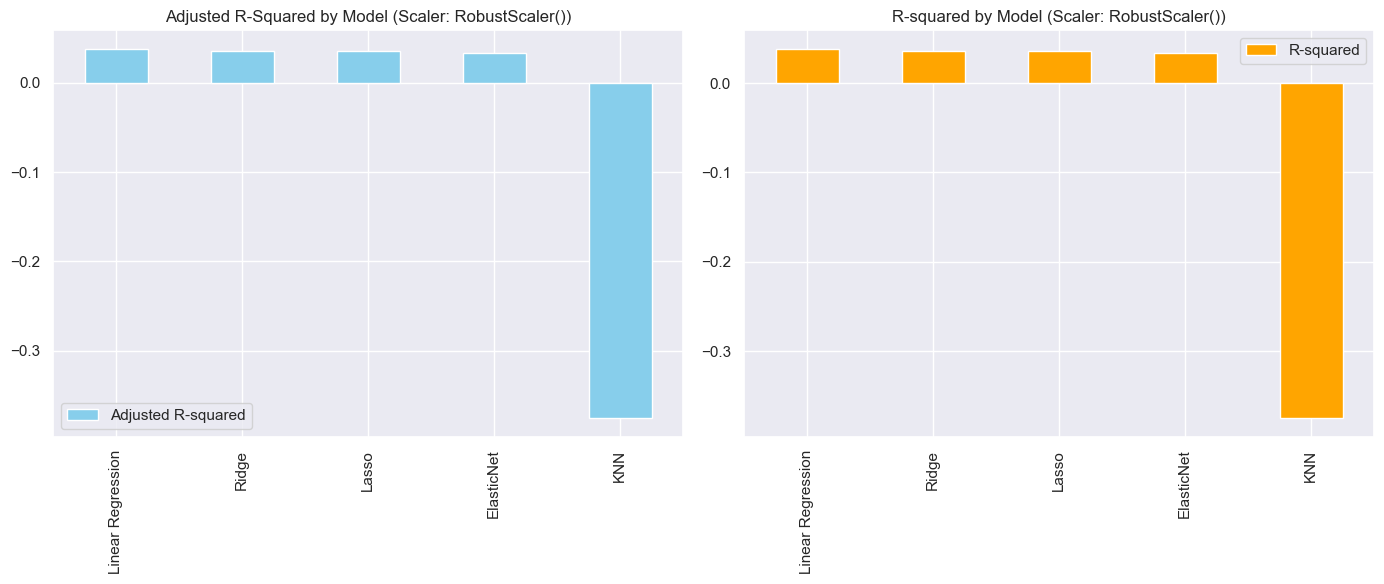
\includegraphics[width=\linewidth]{Images/evalRegModelProviders.png}
\caption{Model Performance for Provider Data}
\label{fig:Robust Scaler Results}
\end{figure}

\begin{table}[ht]
\centering
\begin{tabular}{@{}lrr@{}}
\toprule
Model            & \multicolumn{1}{c}{Adjusted R-squared} & \multicolumn{1}{c}{R-squared} \\ 
\midrule
Linear Regression & 0.037 & 0.038\\
Ridge             & 0.035 & 0.035\\
Lasso             & 0.035 & 0.035\\
ElasticNet        & 0.033 & 0.033\\
KNN               & -0.375 & -0.374\\
\bottomrule
\end{tabular}
\label{tab:model_performance robust}
\end{table}

Following the data presented in Figure 13, which outlines the performance of various regression models using the consolidated provider data, it is evident that the predictive capability of these models is notably limited. The $R^2$ values across all linear models, including Linear Regression, Ridge, Lasso, and ElasticNet, hover around 0.035, suggesting that these models explain a very small fraction of the variance in the net income from the data provided. Notably, the K-Nearest Neighbors (KNN) model performs significantly worse, with an $R^2$ value of approximately -0.375, indicating that the model fits the data even less effectively than a model that simply predicts the mean net income.

\pagebreak
\subsubsection{Descriptive Analytics}
Descriptive analytical methods will be used to profile the provider data of Skilled Nursing Facilities. Although the proivder features may not have strong predictive power for net income, several key features from the dataset can still be leveraged to assess historical operational performance. Operational indicators such as the number of certified beds and average number of residents per day highlight facility utilization rates, while staffing ratings and reported hours provide insight into the quality of care and staffing efficiency, crucial for maintaining high service levels. Furthermore, overall facility ratings and health inspection outcomes serve as direct reflections of a facility's reputation and operational success, influencing both patient outcomes and financial viability.


\begin{figure}[htbp]
\centering
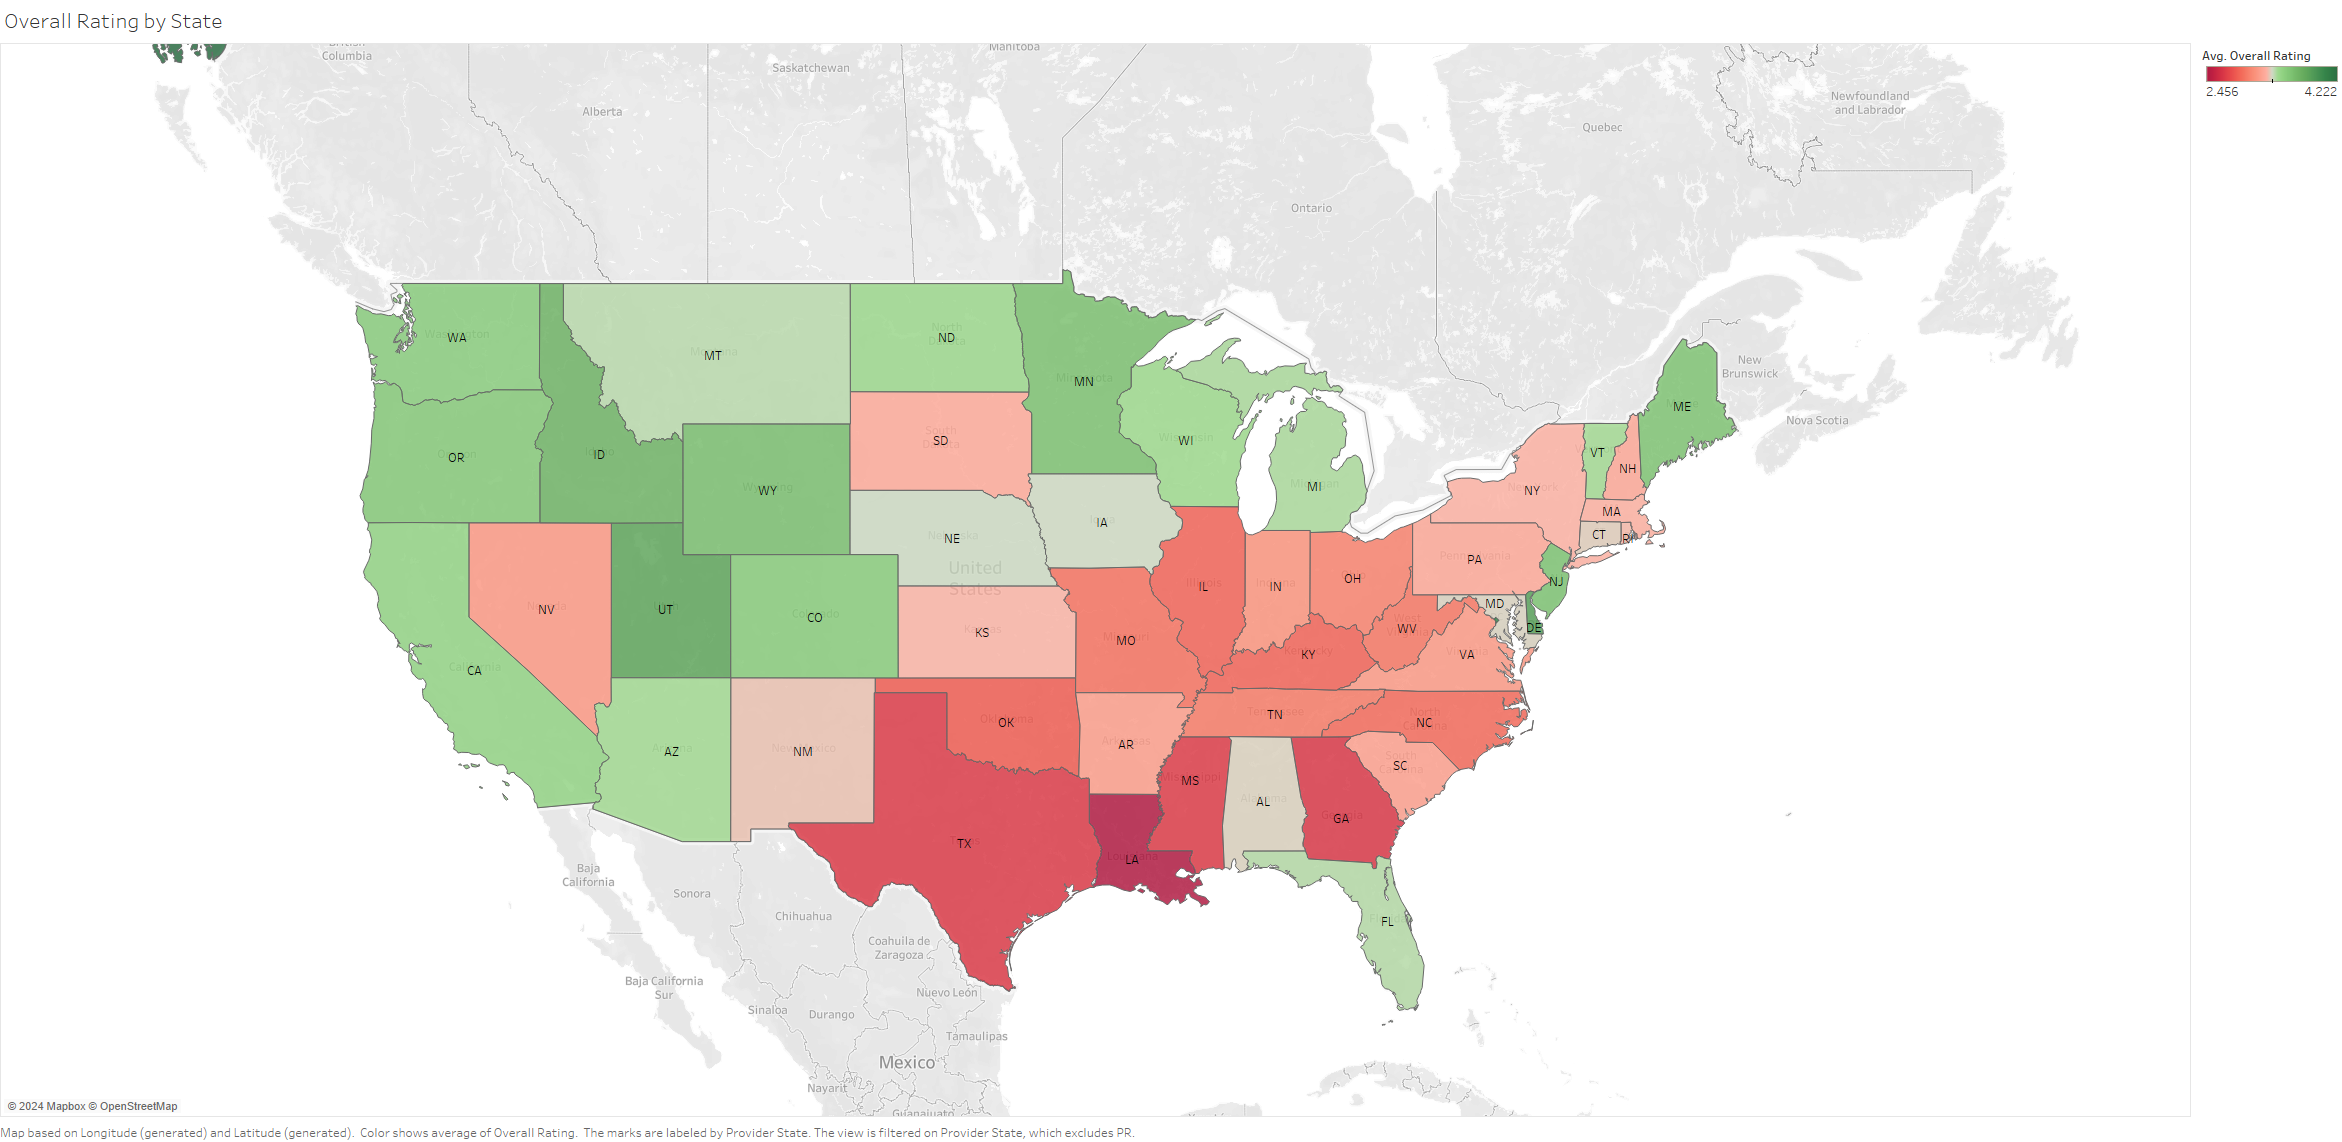
\includegraphics[width=\linewidth]{Images/Overall Rating by State.png}
\caption{Overall Rating by State}
\label{Rating by state}
\end{figure}

\begin{figure}[htbp]
\centering
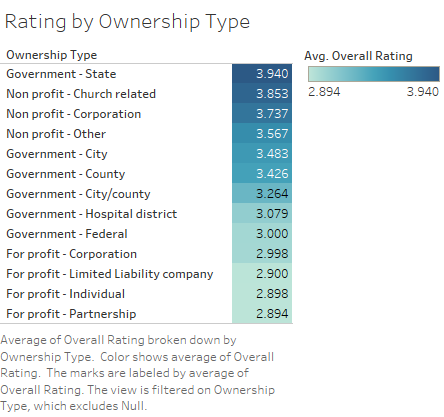
\includegraphics[width=0.4\linewidth]{Images/Rating by Ownership Type.png}
\caption{Overall ratings by ownership type}
\label{ratings by ownership}
\end{figure}

\pagebreak

We found that the strongest single variable to related to overall rating was total reported nursing hours per resident per day. The model used to predict the average overall rating based on average reported total nurse staffing hours per resident per day can be estimated with the following equation:
\begin{equation}
    \text{Avg. Overall Rating} = 2.02 \cdot \ln(\text{Avg. Reported Total Nurse Staffing Hours per Resident per Day}) + 0.482
\end{equation}

The regression results show that the coefficient for the logarithm of average reported total nurse staffing hours per resident per day is highly significant:

\begin{table}[ht]
\centering
\caption{Trend line statistics}
\begin{tabular}{@{}lcccc@{}}
\toprule
Term & Value & StdErr & t-value & p-value \\ 
\midrule
ln(Avg. Reported Total Nurse Staffing Hours per Resident per Day) & 2.02107 & 0.257443 & 7.85055 & \(< 0.0001\) \\
Intercept & 0.481649 & 0.362640 & 1.32818 & 0.190151 \\
\bottomrule
\end{tabular}
\end{table}

\begin{figure}[htbp]
\centering
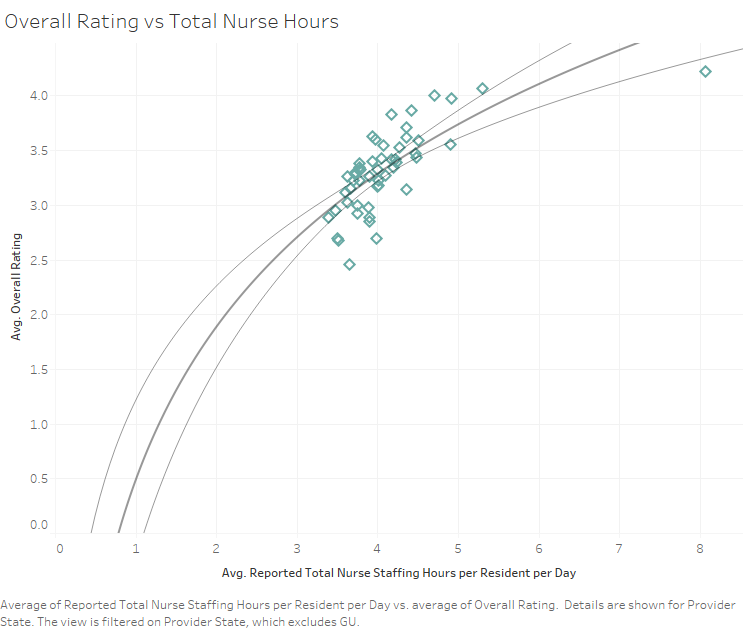
\includegraphics[width=0.7\linewidth]{Images/Overall Rating vs Total Nurse Hours.png}
\caption{Overall Rating vs. Total Nurse Hours per Resident per Day}
\label{Rating by state}
\end{figure}


\pagebreak
Below is our analysis of quality measures, both short and long stay, and the features that were moderately to highly positvely correlated with QM. 
\begin{figure}[htbp]
\centering
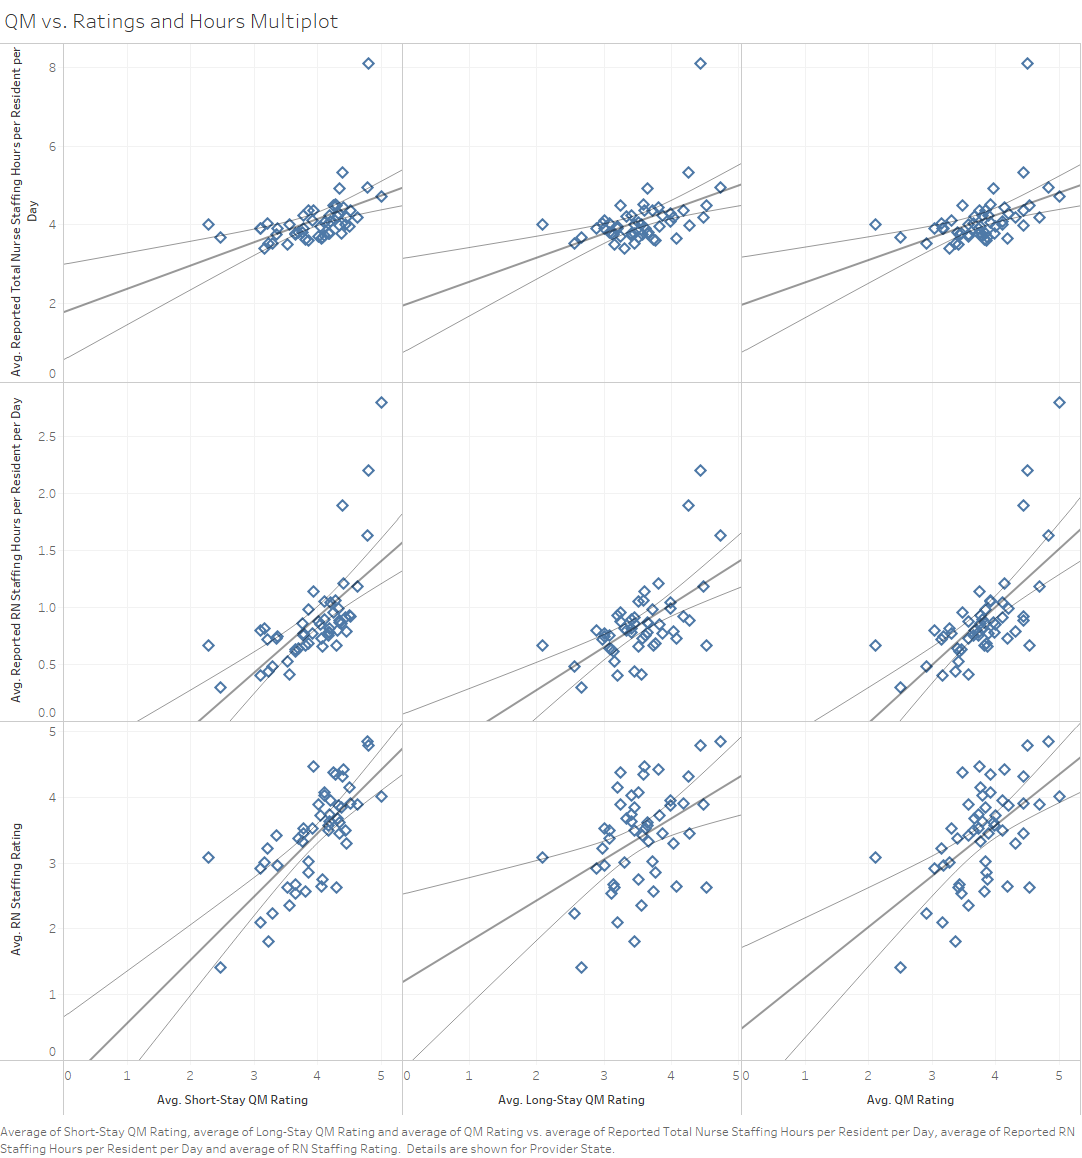
\includegraphics[width=\linewidth]{Images/QM vs. Ratings and Hours Multiplot.png}
\caption{Quality Measures vs Ratings and RN Hours}
\label{fig:provEDA}
\end{figure}
\pagebreak
\subsubsection{Cluster Analysis}
The states were clustered on the basis of overall ratings, RN hours per resident per day, and RN staff rating. Two clusters was the default by Tableau, but three clusters were used instead for interpretability.

\begin{figure}[htbp]
\centering
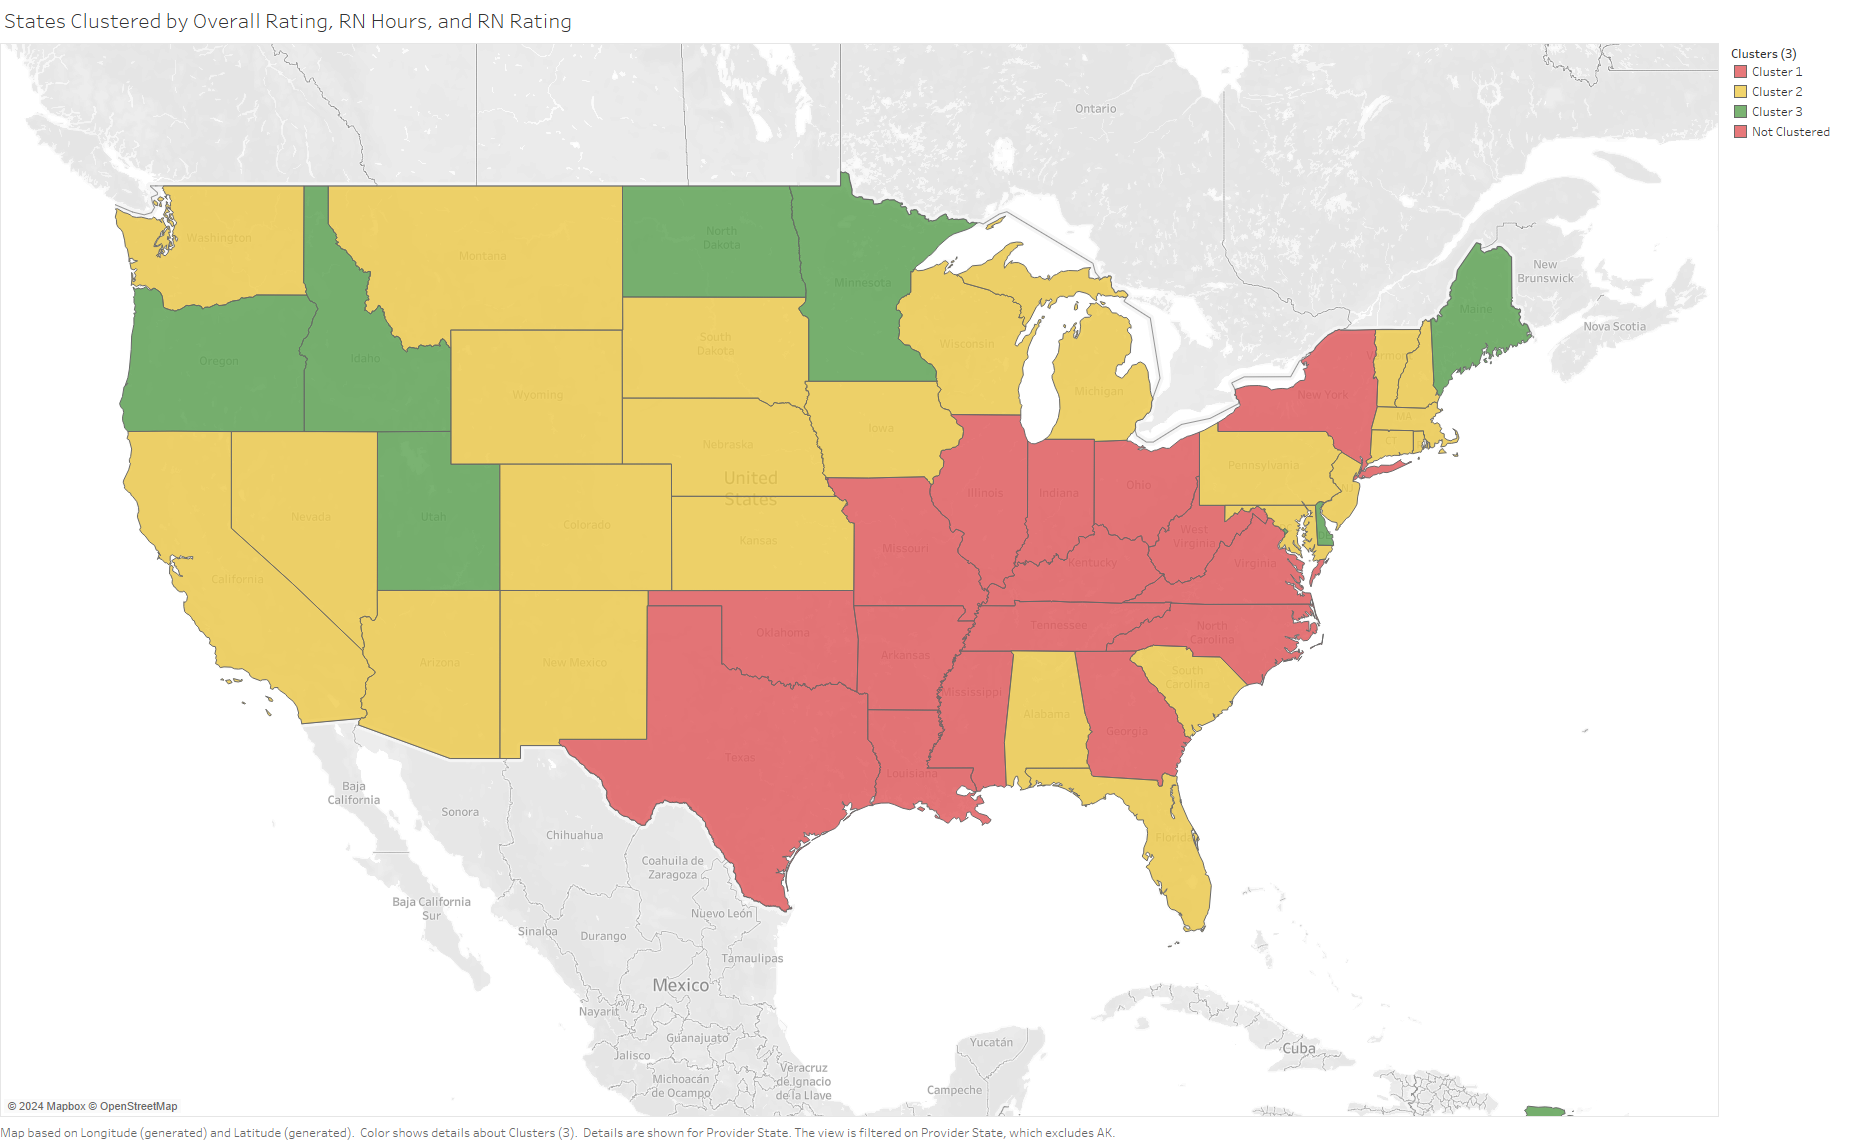
\includegraphics[width=\linewidth]{Images/States Clustered by Overall Rating, RN Hours, and RN Rating.png}
\caption{States clustered by overall Ratings, RN Hours, and RN Ratings}
\label{fig:Clustering by Prov Data}
\end{figure}

\section*{Inputs for Clustering}
\subsection*{Variables}
\begin{itemize}
    \item Avg. Overall Rating
    \item Avg. RN Staffing Rating
    \item Avg. Reported Total Nurse Staffing Hours per Resident per Day
\end{itemize}
\subsection*{Level of Detail}
\begin{itemize}
    \item Provider State
\end{itemize}
\subsection*{Scaling}
\begin{itemize}
    \item Normalized
\end{itemize}

\section*{Clusting Summary}
\begin{tabular}{@{}lr@{}}
\toprule
\textbf{Metric} & \textbf{Value} \\
\midrule
Number of Clusters & 3 \\
Number of Points & 52 \\
Between-group Sum of Squares & 3.8674 \\
Within-group Sum of Squares & 1.9744 \\
Total Sum of Squares & 5.8418 \\
\bottomrule
\end{tabular}


\section*{Analysis of Variance (ANOVA)}
{\footnotesize % Reduces the font size
\begin{tabular}{@{}lllllll@{}}
\toprule
\textbf{Variable} & \textbf{F-statistic} & \textbf{p-value} & \textbf{Model SS} & \textbf{DF} & \textbf{Error SS} & \textbf{DF} \\
\midrule
Avg. RN Staffing Rating & 18.06 & 1.33e-06 & 1.666 & 2 & 2.26 & 49 \\
Avg. Overall Rating & 16.51 & 3.307e-06 & 1.599 & 2 & 2.373 & 49 \\
Avg. Reported Total Nurse Staffing Hours per Resident per Day & 12.21 & 4.968e-05 & 0.6029 & 2 & 1.209 & 49 \\
\bottomrule
\end{tabular}
}

\section*{Cluster Centers}
\begin{tabular}{@{}>{\raggedright\arraybackslash}p{2cm} 
                 >{\raggedright\arraybackslash}p{2cm} 
                 >{\raggedright\arraybackslash}p{3cm} 
                 >{\raggedright\arraybackslash}p{3cm} 
                 >{\raggedright\arraybackslash}p{4cm}@{}}
\toprule
\textbf{Clusters} & \textbf{Number of Items} & \textbf{Avg. Overall Rating} & \textbf{Avg. RN Staffing Rating} & \textbf{Avg. Reported Total Nurse Staffing Hours per Resident per Day} \\
\midrule
Cluster 1 & 16 & 2.9163 & 2.5251 & 3.7051 \\
Cluster 2 & 25 & 3.3567 & 3.5675 & 4.0001 \\
Cluster 3 & 11 & 3.6924 & 4.2849 & 4.8561 \\
\bottomrule
\end{tabular}

\section*{Provider State Clusters}

\begin{tabular}{@{}ll@{}}
\toprule
\textbf{Cluster 2} & \textbf{Cluster 3} \\
\midrule
AL & DC \\
AZ & DE \\
CA & GU \\
CO & HI \\
CT & ID \\
FL & ME \\
IA & MN \\
KS & ND \\
MA & OR \\
MD & PR \\
MI & UT \\
MT &  \\
NE &  \\
NH &  \\
NJ &  \\
NM &  \\
NV &  \\
PA &  \\
RI &  \\
SC &  \\
SD &  \\
VT &  \\
WA &  \\
WI &  \\
WY &  \\
\end{tabular}

\pagebreak
With the clusters created, we profiled the clusters by the number of certified beds. This distribution was analyzed by using box plots and below are the results. 
\begin{figure}[htbp]
\centering
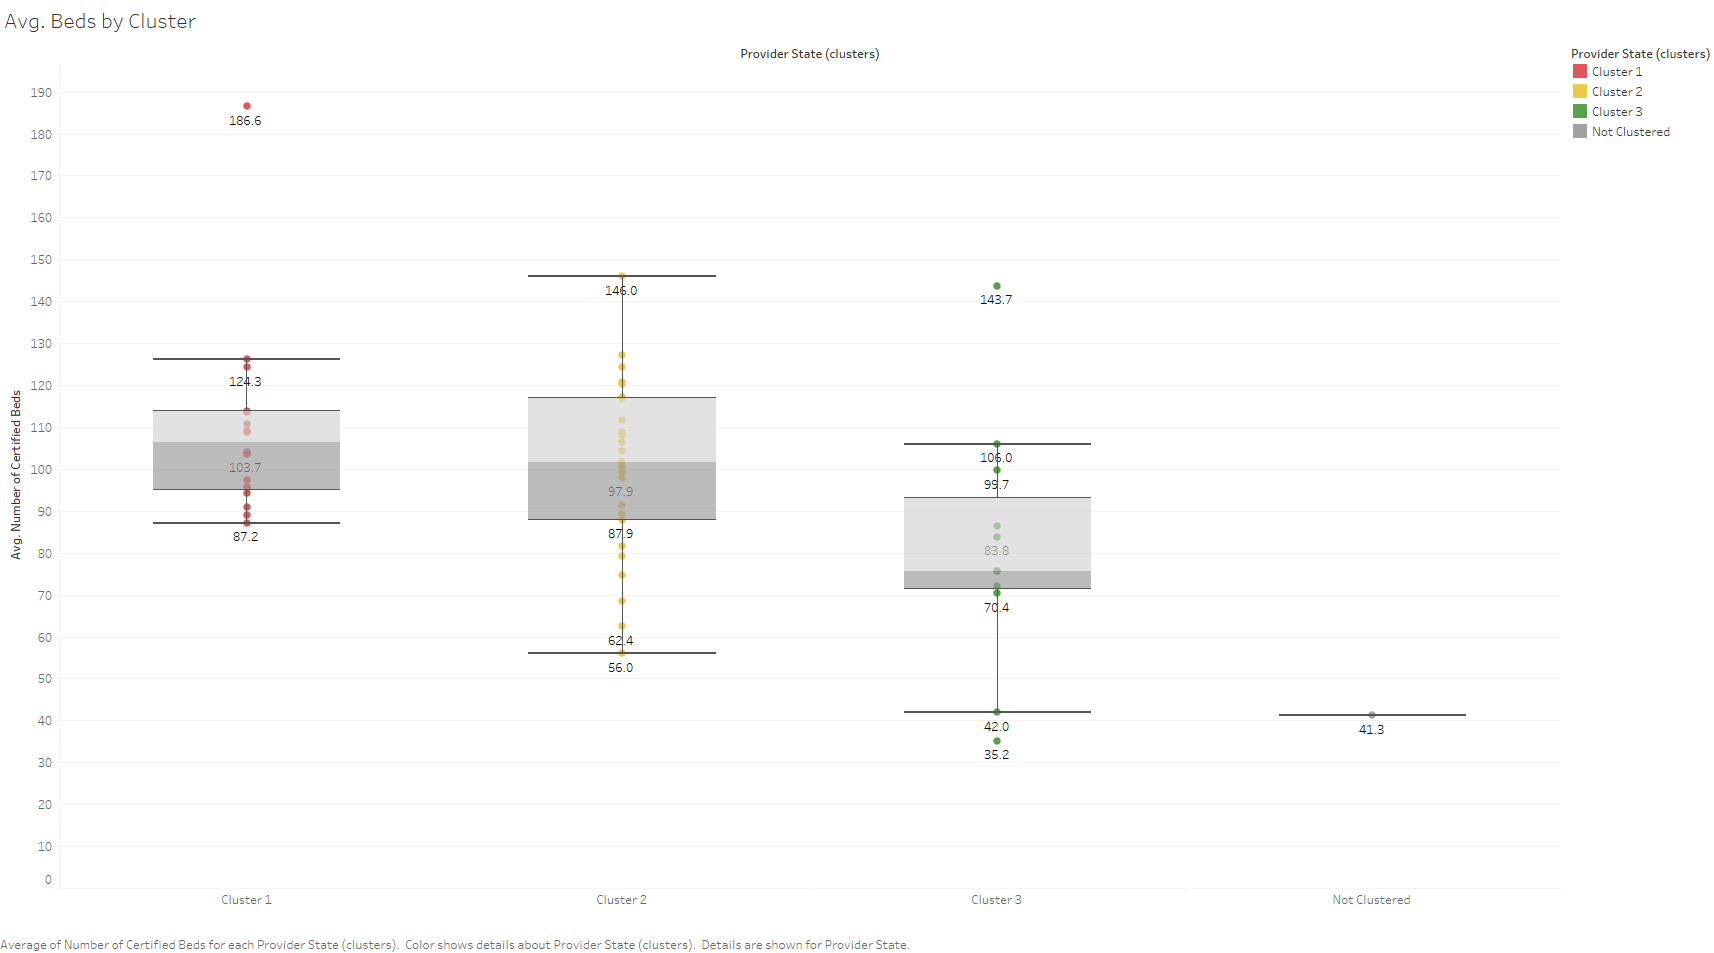
\includegraphics[width=\linewidth]{Images/Avg. Beds by Cluster.png}
\caption{Distribution of certified beds by cluster by state}
\label{bed dist.}
\end{figure}




\pagebreak

\subsection{COVID-19 Data}
As foreshadowed by the scatter plots in the EDA section for COVID, the vaccination rates are not strong indicators of net income. The models are contained in the source code of  this project repository for reference, but will be excluded in this report. Therefore, to analyze the financial and operational effects of COVID on Skilled Nursing Facilities, descriptive analytics will be used instead. 

We will define all years 2019 and after as COVID years, and all previous years as non-COVID years. Data from both previously utilized sources, the cost reports and the provider data, will be plotted overtime to uncover changes between non-COVID and COVID years.


\begin{figure}[htbp]
\centering
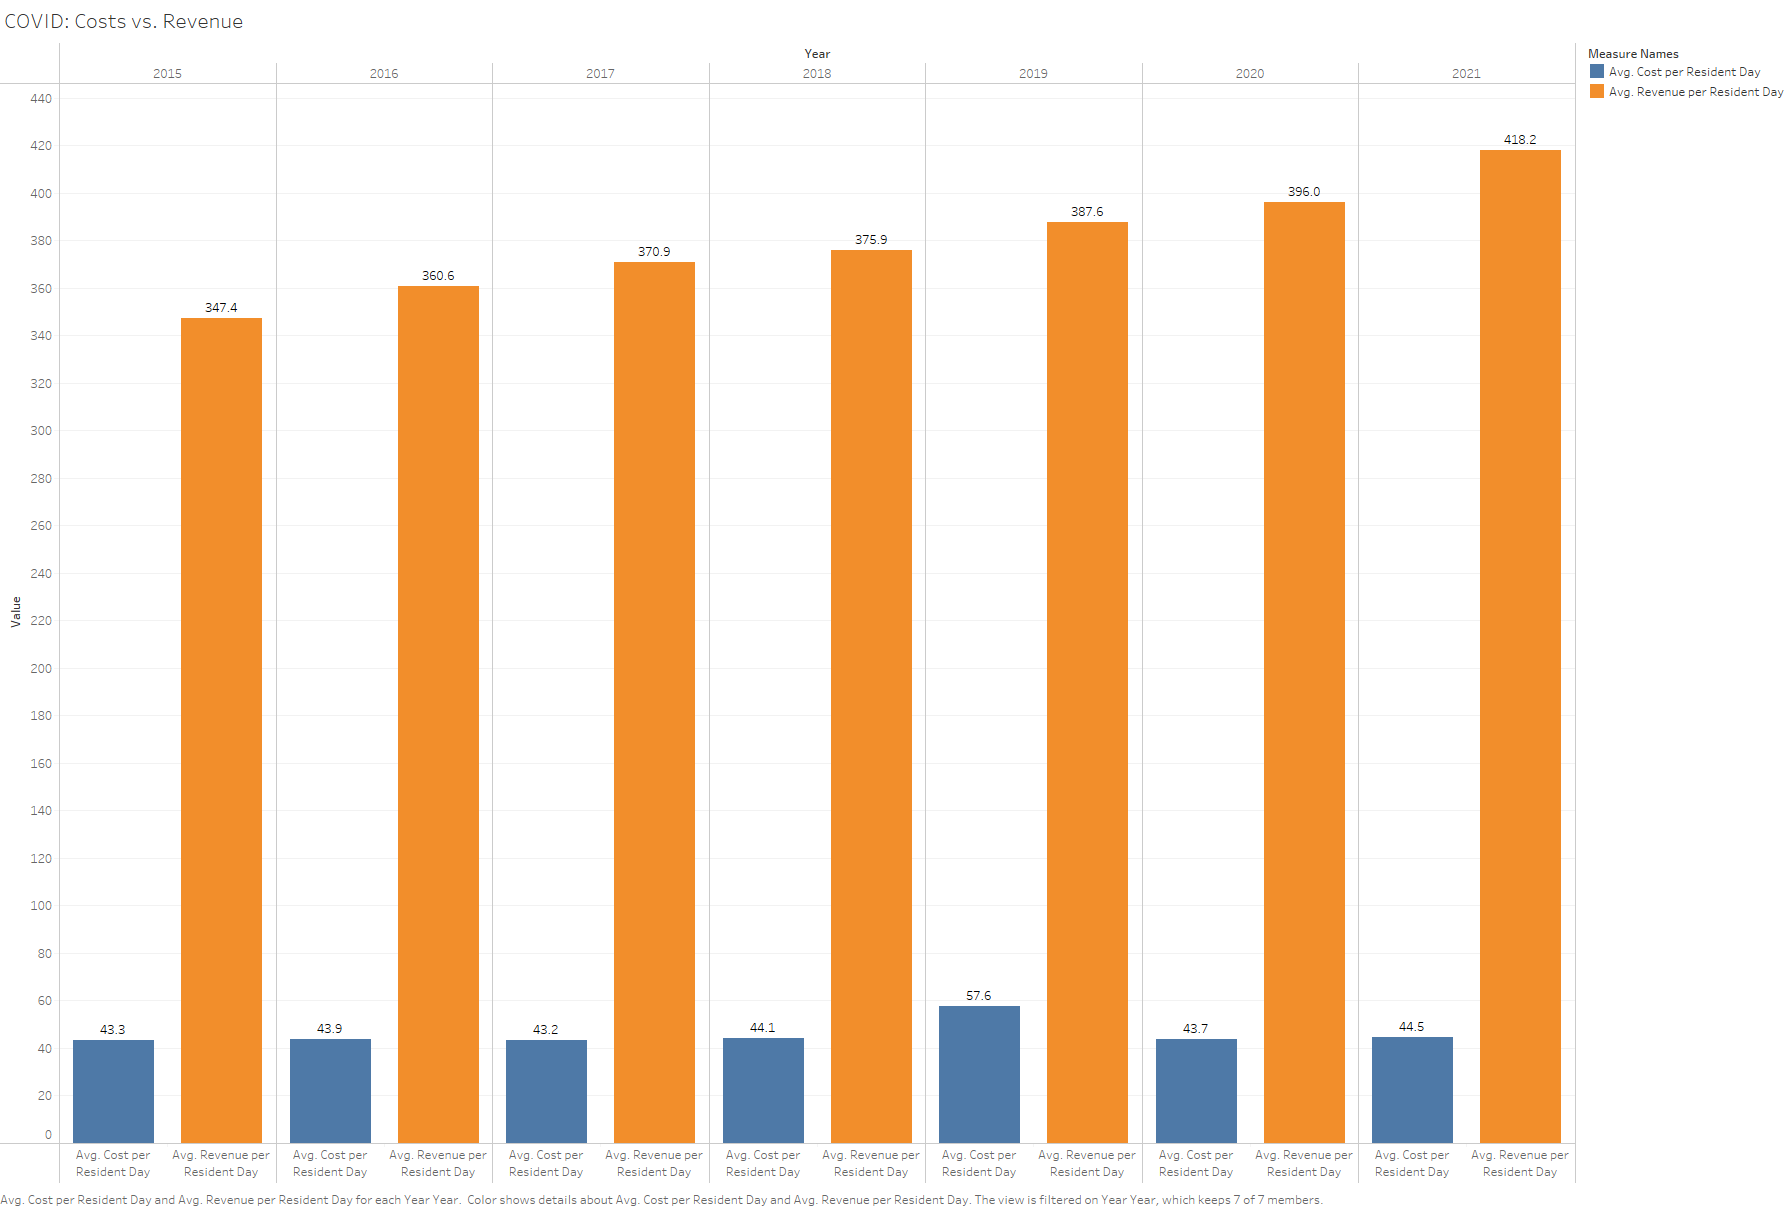
\includegraphics[width=\linewidth]{Images/COVID Costs vs. Revenue.png}
\caption{Costs \& Revenue Per Resident Day Over Time}
\label{fig:Robust Scaler Results}
\end{figure}

\noindent The calculated fields are defined by the following:

\[\text{Cost per resident day = }\frac{\text{Total Cost}}{\text{Total Days Total}}\]

\[\text{Revenue per resident day = }\frac{\text{Gross Revenue}}{\text{Total Days Total}}\]

\noindent Total Days Total represents the number of inpatient days or visits, where applicable, for all programs combined.

\pagebreak
\begin{figure}[htbp]
\centering
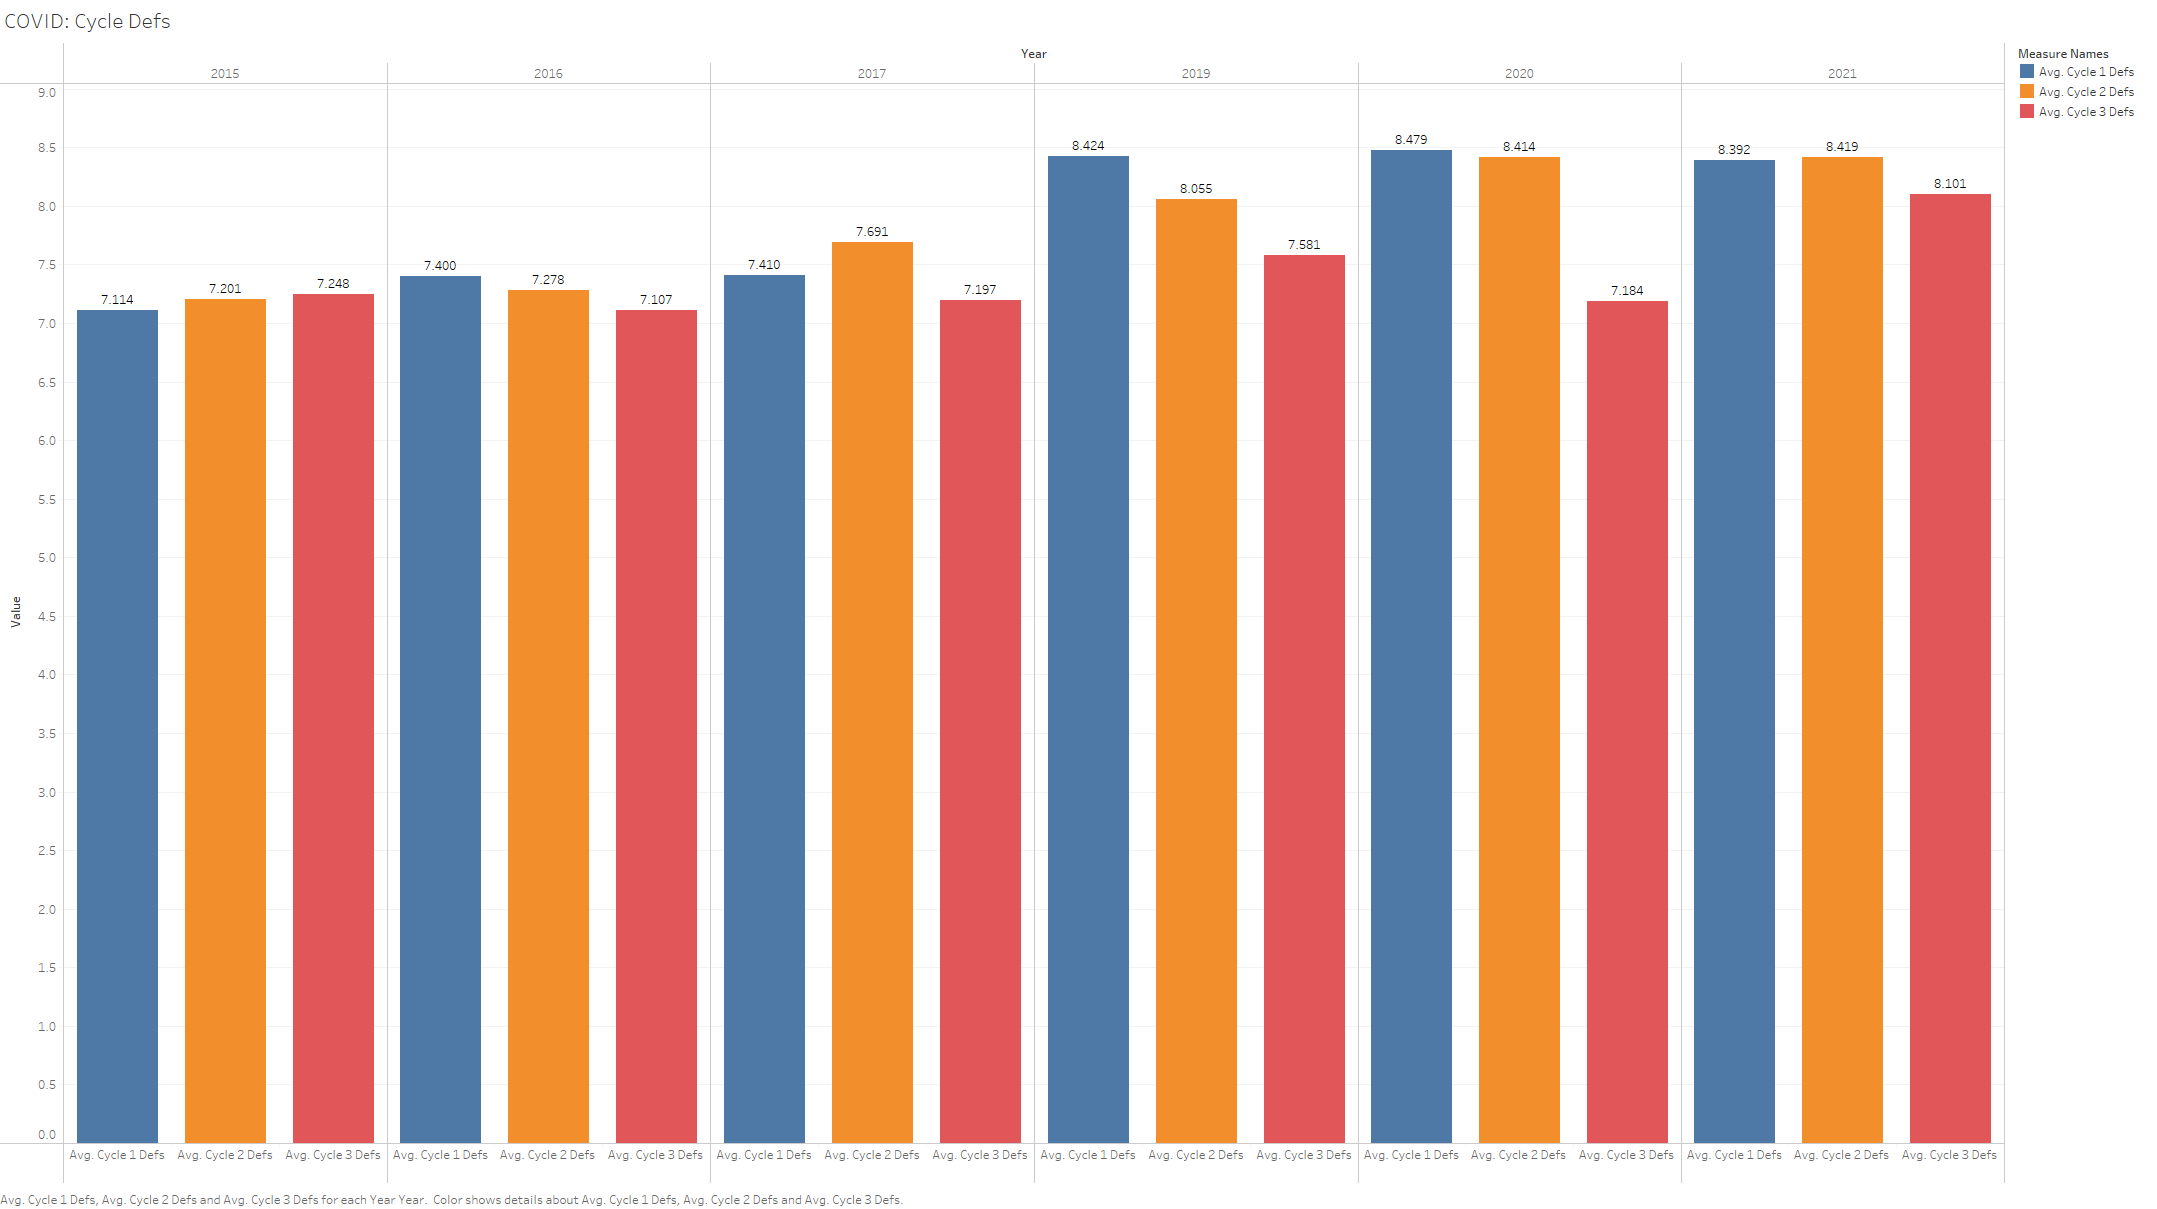
\includegraphics[width=\linewidth]{Images/COVID Cycle Defs.png}
\caption{Average Cycle Deficiency Counts Over Time}
\label{defs over time}
\end{figure}

CMS calculates a total weighted health inspection score for each facility (including any repeat revisits). 
Note that a lower survey score corresponds to fewer deficiencies and revisits, and thus better performance 
on the health inspection domain. In calculating the total weighted score, more recent standard surveys are 
weighted more heavily than earlier surveys with the most recent period (rating cycle 1) being assigned a 
weighting factor of 1/2, the previous period (rating cycle 2) having a weighting factor of 1/3, and the 
second prior period (rating cycle 3) having a weighting factor of 1/6. The individual weighted scores for 
each cycle are then summed (after including complaint surveys, focused infection control surveys, and 
revisit points) to create the total weighted health inspection score for each facility. 

\pagebreak
\begin{figure}[htbp]
\centering
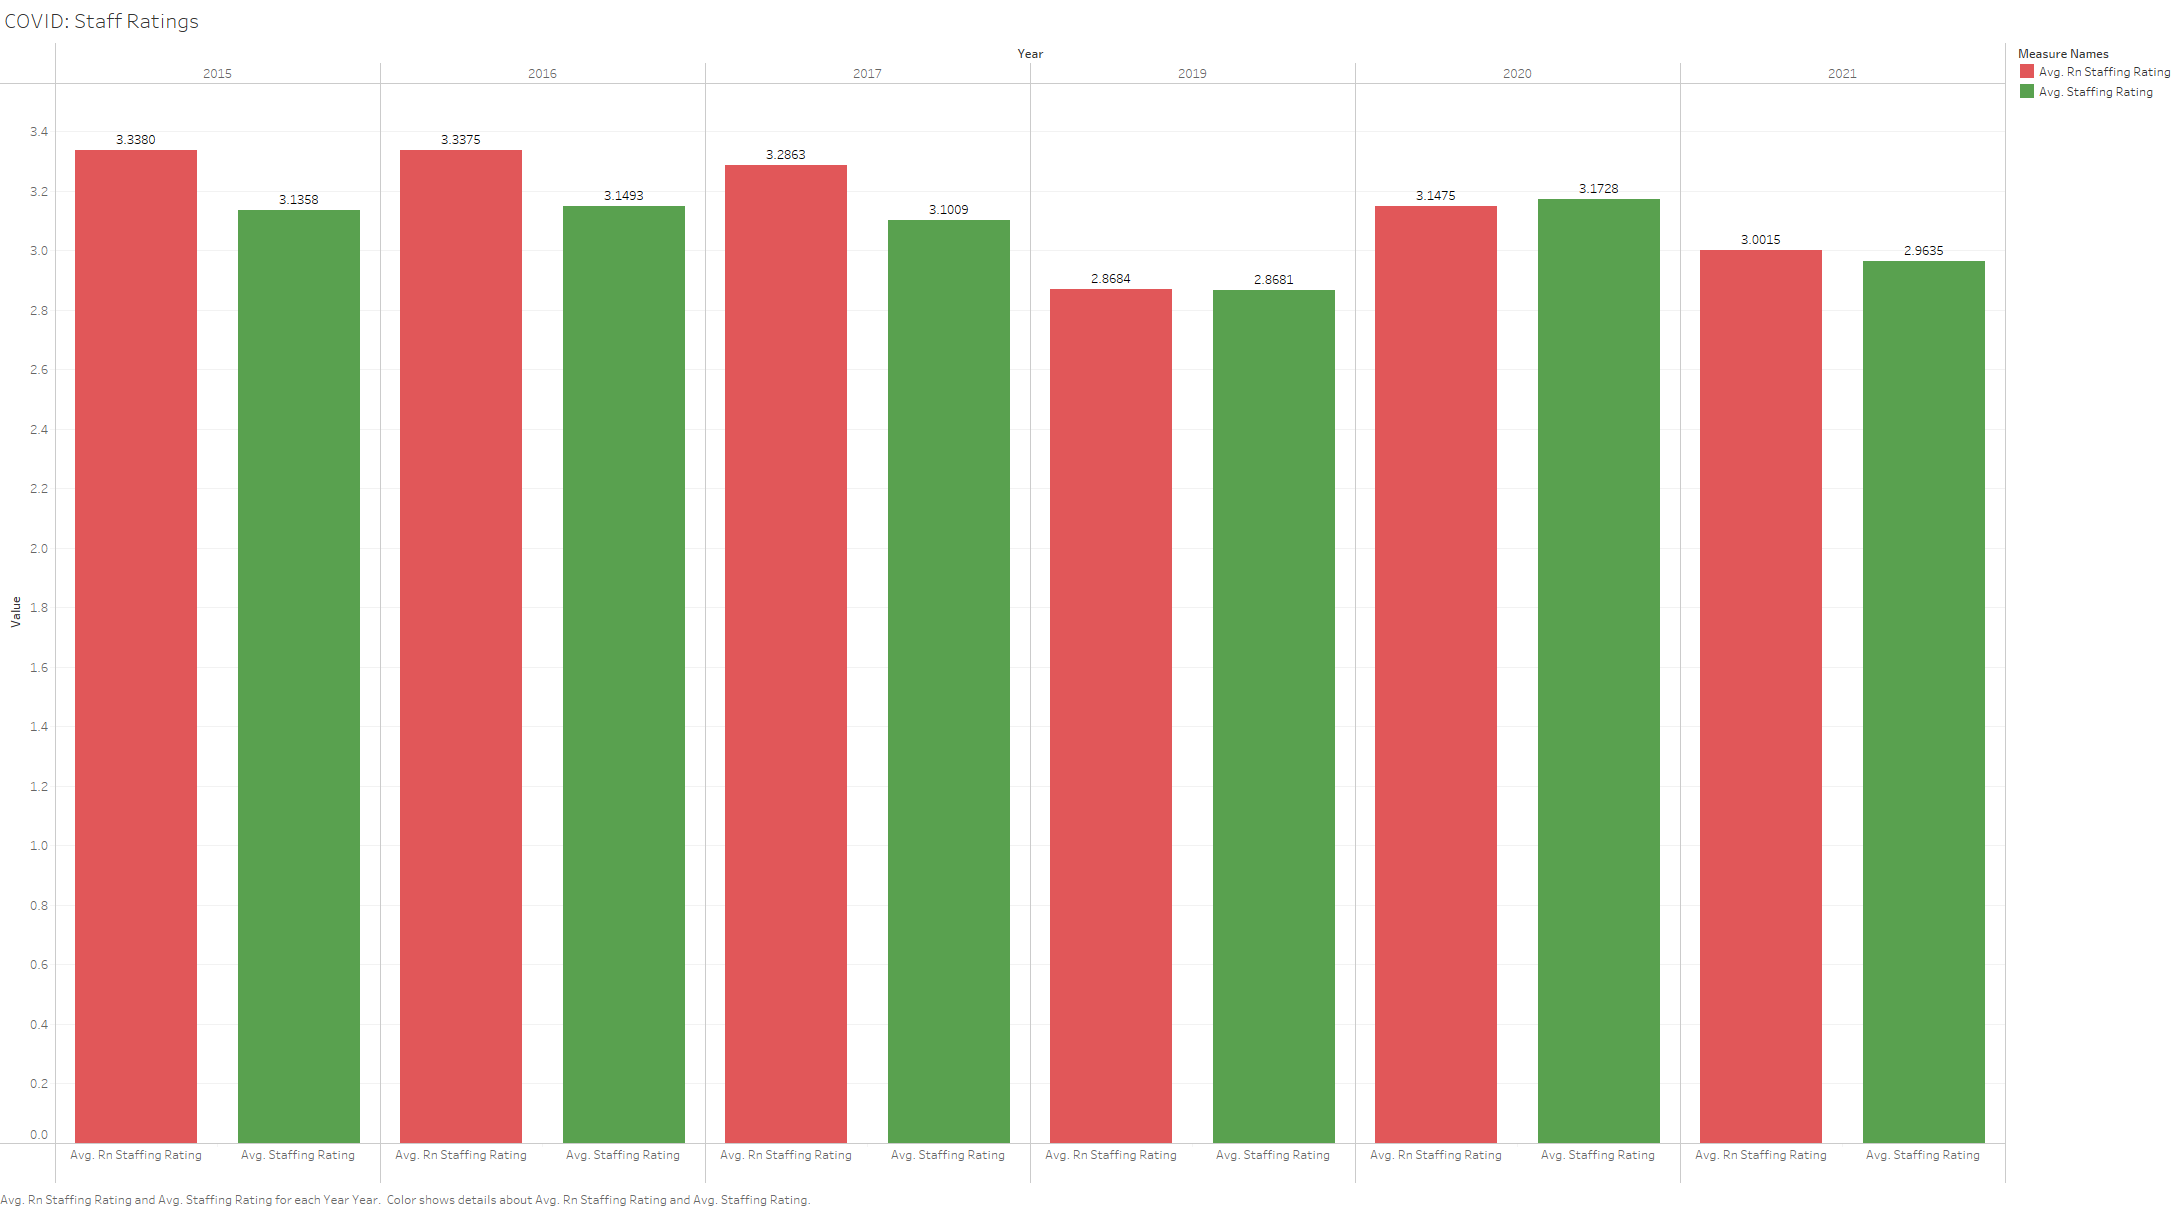
\includegraphics[width=\linewidth]{Images/COVID Staff Ratings.png}
\caption{Average Staff Ratings Over Time}
\label{ratings over time}
\end{figure}

\noindent Average staff ratings also changed over time. There is a clear decrease in staff ratings from non-COVID-19 years and COVID-19 years. 




\pagebreak
%-------------------END: Analysis and Findings------------------------------------
%-------------------BEGIN: Discussion------------------------------------

\section{Discussion}
The project objectives are to determine feasibility behind investing in skilled nursing facilities and what markets to invest into. From the exploratory data analysis, we observed that net income from skilled nursing facilities is, on average, increasing across all states within the period. The regression analysis of the cost report data found the most important features for predicting net income and the cluster analysis found which markets perform the best with respect to these features and quality ratings. The strongest predictors of net income were total assets, inpatient pps amount, overhead (non-salary), total liabilites and fund balances, less total operating expsenses, total salaries, and net profit margin. The CMS Five-Star Quality Rating System uses an algorithm that incorporates health inspection measures, staffing measure, and quality measures to determine an overall rating. This overall rating provides consumers with an at-a-glance method to determine if a particular nursing home is sufficient for them. By using the overall rating, total RN hours per resident per day, and RN staffing rating, the states were clustered again. From both sets of cluster analysis, it was found that Arizona (AZ), California (CA), Connecticut (CT), District of Columbia (DC), Delaware (DE), Hawaii (HI), Maryland (MD), New Jersey (NJ), and Nevada (NV) were the states that performed best in 2021 in terms of financial predictors of net income and quality ratings. 

\subsection{Impact of COVID-19 on Skilled Nursing Facilities}
We found that average revenue per resident day has been increasing over time, going from \$347, \$360, \$370, \$375, \$387, \$396, to \$418. We also found that average cost per resident day increased  to \$57 during 2019, likely due to increased cost of PPE and over time hours spent to staffing, but since then has stayed around \$44. However, another study found that operating margins decreased by approximately 4.5\% while operating costs per resident increased by \$26.51, outweighing the increase in operating revenue per resident day by about \$17\textsuperscript{\cite{orewa2024}}.

It was also found that COVID-19 years had a significant increase in deficiencies compared to non-COVID-19 years. This can likely be attributed to harsher inspection standards as a result of COVID-19. Staff ratings had also decreased on average after COVID-19, likely due to harsher quality standards and increased stress by health service staff.   

\subsection{Limitations}

This study is subject to the constraints of data availability and currency. The time period analyzed was from 2015 through 2021. Therefore, recent trends and developments from 2021 through 2023 are not captured. This study did not account for inflation adjustments in the financial records examined. It is possible that more critical predictors of financial performance were either not available within the datasets used or were overlooked in the analysis. Furthermore, there is a growing amount of literature sugguesting the possibility that nursing homes may be concealing profits through transactions involving related parties\textsuperscript{\cite{harrington2024united}}. The accuracy of the findings of this study is contingent upon the precision of the financial reporting by the nursing homes. 

This study was conducted from a nationwide perspective and latent trends within specific states were not explored. For instance, regression alaysis from another study on specifically California  found that the number of beds, occupancy rates, high-quality rating scores, and medium and high proportions of Medicare resident days were positively associated with net income margins in 2019 and 2020.\textsuperscript{\cite{Harrington2023}}. 

\pagebreak
%-------------------END: Discussion------------------------------------
%-------------------BEGIN: Recommendations------------------------------------
\section{Recommendations}
% Based on the analysis and findings, provide actionable recommendations for the business. Clearly articulate the expected impact of these recommendations and suggest a plan for implementation.

More studies on skilled nursing facilities within a subset of states are needed to closely examine trends overtime. Studies should target one or more of the following states: Arizona (AZ), California (CA), Connecticut (CT), District of Columbia (DC), Delaware (DE), Hawaii (HI), Maryland (MD), New Jersey (NJ), and Nevada (NV). For instance, the Public Policy Institute of California had found that most regions would need to increase capacity to meet projected demand of skilled nursing homes\textsuperscript{\cite{ppic2024}}. This is in contrast from what has found by a study from KFF which found that there has been a 4\% closure in nursing facilities and 12\% reduction in residents from 2015 to 2023\textsuperscript{\cite{kff2024}}. Additional and further studies should analyze patterns and trends within specific cities and counties. These studies should utilize additional demographic data to make a data driven decision behind skilled nuring facility investment. 


\pagebreak
%-------------------END: Recommendations------------------------------------
%-------------------BEGIN: Conclusion------------------------------------
\section{Conclusion}
This comprehensive study has effectively explored the financial and operational dynamics of skilled nursing facilities across the United States from 2015 through 2021, yielding critical insights that can guide investment decisions in this sector. The analysis revealed that net income across skilled nursing facilities is on an upward trend, underpinned by a set of key financial and operational metrics. Notably, total assets, inpatient PPS amount, and net profit margins emerged as pivotal predictors of financial performance.

The application of cluster analysis further delineated the markets that showcase optimal performance, highlighting states like Arizona, California, Connecticut, and others as prime candidates for potential investments due to their robust financial and quality metrics. 

The COVID-19 pandemic introduced additional complexities, influencing both the operational costs and the overall financial performance of nursing facilities. The data indicated shifts in costs and revenue streams during the pandemic years, with a notable impact on staffing and health inspection scores.


\pagebreak
%-------------------END: Conclusion------------------------------------
%-------------------BEGIN: Appendices------------------------------------
\section{Appendices}
Please refer to my project's GitHub repository for the source code and additional resources at \href{https://github.com/Musiik-fn/620-Project-Codebase}{this link}! Nearly all the work related to this project was tracked using git, and therefore, the versioning, commit history, and overall progression of the project is visbile at the linked repo. If visiting the repository, the files of interest would be of the extensions .ipynb, .tex, and .twb. 
%-------------------END: Appendices------------------------------------

\pagebreak
%-------------------BEGIN: References------------------------------------
\section{References}

\begin{thebibliography}{9}

\bibitem{hughes2023rates}
Hughes, K., Feng, Z., Li, Q., Segelman, M., Oliveira, I., \& Dey, J. G. (2023).
\textit{Rates of nursing home closures were relatively stable over the past decade, but warrant continuous monitoring}.
Health Affairs Scholar, 1(2), qxad025. Oxford University Press US. Available online: \href{https://scholar.google.com/scholar_lookup?journal=Heal+Aff+Sch&title=Rates+of+nursing+home+closures+were+relatively+stable+over+the+past+decade,+but+warrant+continuous+monitoring&author=K+Hughes&author=Z+Feng&author=Q+Li&volume=1&issue=2&publication_year=2023&d=gs_cit&t=1714807740518&u=%2Fscholar%3Fq%3Dinfo%3AT6cB2hNX4sgJ%3Ascholar.google.com%2F%26output%3Dcite%26scirp%3D0%26hl%3Den}{Google Scholar}.

\bibitem{tyler2017rebalance}
Denise A. Tyler and Mary L. Fennell.
\textit{Rebalance without the balance: A research note on the availability of community-based services in areas where nursing homes have closed}.
Research on Aging, 39(5): 597--611, 2017.
SAGE Publications Sage CA: Los Angeles, CA. Available online: \href{https://scholar.google.com/scholar_lookup?journal=Heal+Aff+Sch&title=Rates+of+nursing+home+closures+were+relatively+stable+over+the+past+decade,+but+warrant+continuous+monitoring&author=K+Hughes&author=Z+Feng&author=Q+Li&volume=1&issue=2&publication_year=2023&}{Google Scholar}.

\bibitem{sklearn}
scikit-learn developers. 
\textit{scikit-learn: Machine Learning in Python}. 
2021. 
\url{https://scikit-learn.org}

\bibitem{cms2023}
Centers for Medicare \& Medicaid Services.
\textit{CMS Cost Reports}. 
Available at: \url{https://www.cms.gov/data-research/statistics-trends-and-reports/cost-reports}.
Accessed: [2024-05-04].

\bibitem{cmsfive2023}
Centers for Medicare \& Medicaid Services.
\textit{Five-Star Quality Rating System}. 
Available at: \url{https://www.cms.gov/medicare/health-safety-standards/certification-compliance/five-star-quality-rating-system}.
Accessed: [2024-05-04].

\bibitem{cmsqso2313}
Centers for Medicare \& Medicaid Services.
\textit{QSO-23-13-ALL}. 
Available at: \url{https://www.cms.gov/files/document/qso-23-13-all.pdf}.
Accessed: [2024-05-04].

\bibitem{harrington2024united}
Charlene Harrington, Richard Mollot, Robert Tyler Braun, and Dunc Williams Jr.
\textit{United States' nursing home finances: spending, profitability, and capital structure}.
International Journal of Social Determinants of Health and Health Services, 54(2):131--142, 2024.
SAGE Publications Sage CA: Los Angeles, CA.

\bibitem{Harrington2023}
Harrington, C.A., Hailer, L., Mollot, R.J., Mukamel, D.B. 
\textit{Examining California nursing home profitability and related factors before and during the COVID-19 pandemic}.
Journal of the American Geriatrics Society, 71(8), 2530-2538. 
\url{https://doi.org/10.1111/jgs.18356} (2023, April 7). PMID: 37026588.

\bibitem{provCMS}
Centers for Medicare \& Medicaid Services. (2023).
\textit{Nursing Home Data Compendium}.
Available at: \url{https://www.cms.gov/medicare/provider-enrollment-and-certification/certificationandcomplianc/downloads/usersguide.pdf} [Accessed: 10 May 2024].

\bibitem{orewa2024}
Orewa, G. N., Weech-Maldonado, R., Lord, J., Davlyatov, G., Becker, D., \& Feldman, S. S. (2024).
\textit{COVID-19 Pandemic Impact on Nursing Homes Financial Performance}.
Inquiry, 61: 00469580241240698. Published online March 21, 2024. doi: \href{https://doi.org/10.1177/00469580241240698}{10.1177/00469580241240698}.
PMCID: PMC10958812, PMID: 38515246.

\bibitem{ppic2024}
Public Policy Institute of California. (2024).
\textit{Anticipating Changes in Regional Demand for Nursing Homes}.
Available at: \url{https://www.ppic.org/publication/anticipating-changes-in-regional-demand-for-nursing-homes/} [Accessed: 10 May 2024].

\bibitem{kff2024}
Kaiser Family Foundation. (2024).
\textit{A Look at Nursing Facility Characteristics}.
Available at: \url{https://www.kff.org/medicaid/issue-brief/a-look-at-nursing-facility-characteristics/} [Accessed: 10 May 2024].

\end{thebibliography}


%-------------------END: References------------------------------------



\end{document}